\chapter{数列的极限}

\section{数列的极限概念}
在前一章中,我们已经看到任何一个实数都可以用有理数来左、右夹逼,即对于任何实数 $x$ 我们总可以用逼近法求得两个有理数列 $\{a_n\}$, $\{b_n\}$ 使得
\[a_1\leqslant a_2\leqslant \cdots \leqslant a_n\leqslant \cdots\leqslant x\leqslant \cdots\leqslant b_n\leqslant \cdots\leqslant b_2\leqslant b_1\]
并且 $b_n-a_n$ 可以小到任意小。

数列中的项 $a_n$ 和 $b_n$ 就是 $x$ 的第 $n$ 次不足近似值和过剩近似值,它们的误差可以用不等式
\[|x-a_n|<b_n-a_n,\qquad |x-b_n|<b_n-a_n\]
来估计。这里所说的逼近的要点在于\emph{误差可以小到任意小},下面用例子从另一个角度来说明这一点。

\medskip
今以 $\dfrac{2}{3}$ 为例,作上述分析:

\medskip
\begin{enumerate}
  \item 以 3 去除 2,得:
    \begin{center}
      \longdivision[2]{2.00}{3}      
    \end{center}
    因为每次 20 除以 3 都余 2, 所以商数 6 重复出现,这个除法可以无止境地作下去。
    \item 上述除式的意义是
\[\begin{split}
    2&=0.6\times3+0.2\Longleftrightarrow 0.6<\frac{2}{3}<0.7,\\
&=0.66\times3+0.02\Longleftrightarrow 0.66<\frac{2}{3}<0.67,\\
&=0.666\times3+0.002\Longleftrightarrow 0.666<\frac{2}{3}<0.667,\\
\cdots 
\end{split}\]
\end{enumerate}

{\linespread{1.6}\selectfont 从上面的分析,同学们可以看出 $\dfrac{2}{3}$ 显然不能用有限位小数表示出,但是存在着由有限位小数所成的无穷数列 $\{a_n\}$ 和 $\{b_n\}$\par}
\[\begin{split}
    \{a_n\}&:\quad a_1=0.6,\; a_2=0.66,\; a_3=0.666,\; \ldots ,\; a_n=0.\underbrace{66\cdots66}_{\text{$n$ 位小数}},\; \ldots\\
    \{b_n\}&:\quad b_1=0.7,\; b_2=0.67,\; b_3=0.667,\; \ldots ,\; b_n=0.\underbrace{66\cdots67}_{\text{$n$ 位小数}},\; \ldots
\end{split}\]
满足 
\[a_n=0.\underbrace{66\cdots66}_{\text{$n$ 位小数}}<\frac{2}{3}<0.\underbrace{66\cdots67}_{\text{$n$ 位小数}}=a_n+\frac{1}{10^n}\]
{\linespread{1.60}\selectfont 并且 $a_n$ 与 $\dfrac{2}{3}$ 之间的误差 $\left|a_n-\dfrac{2}{3}\right|<b_n-a_n=\dfrac{1}{10^n}$, 同样 $b_n$ 与 $\dfrac{2}{3}$ 之间误差 $\left|b_n-\dfrac{2}{3}\right|<\dfrac{1}{10^n}$,只要 $n$ 充分大,误差可以小到任意小。上面的逼近过程,表明无穷数列 $\{a_n\}$, $\{b_n\}$ 从左、右两方面趋近 $\dfrac{2}{3}$,可以使其误差任意小,$\dfrac{2}{3}$ 就是数列 $\{a_n\}$ 的极限,也是数列 $\{b_n\}$ 的极限,用符号表示就是\par}
\[\lim_{n\to\infty}a_n=\frac{2}{3},\qquad \lim_{n\to\infty}b_n=\frac{2}{3}\]
或者用
\[a_n\to \frac{2}{3},\qquad b_n\to\frac{2}{3},\qquad a_n\to \frac{2}{3}\leftarrow b_n\]
来生动地表述上述事实。

{\linespread{1.60}\selectfont 从这里我们看到逼近与极限是密切相关的,极限只是把逼近过程推进到无穷 $(n\to\infty)$ 的结果,逼近只要误差小到所要求的精确度后就可以停止。$\lim\limits_{n\to\infty}a_n=\dfrac{2}{3}$ 表示数列 $\{a_n\}$ 当 $n$ 无限增大的极限值是 $\dfrac{2}{3}$。\par}

{\linespread{1.65}\selectfont
我们再用极限的观点对 $\sqrt{2}$ 进行分析如下。$\sqrt{2}$ 是一个什么数?要回答这个问题,我们只须找出有理数 $\dfrac{a}{b}$ 在什么时候大于 $\sqrt{2}$, 什么时候小于 $\sqrt{2}$,也就是说,如果 $\left(\dfrac{a}{b}\right)^2<2$, 那么正数 $\dfrac{a}{b}<\sqrt{2}$;如果$\left(\dfrac{a}{b}\right)^2>2$, 那么 $\dfrac{a}{b}>\sqrt{2}$。根据有理数是有序的,稠密的,因此有理数的平方总能和 2 比较大小,这就保证我们可以用逼近法(譬如十分逼近法)决定左、右夹逼 $\sqrt{2}$ 的两个由十进位小数组成的数列 $\{a_n\}$、$\{b_n\}$ 如下:\par}
\[\begin{split}
  \{a_n\}&:\quad a_1=1,\; a_2=1.4,\; a_3=1.41,\; a_4=1.414,\ldots\\
  \{b_n\}&:\quad b_1=2,\; b_2=1.5,\; b_3=1.42,\; b_4=1.415,\ldots\\
\end{split}\]
使得 $a_n<\sqrt{2}<b_n$, 而且 $b_n-a_n=\dfrac{1}{10^n}$,于是
\[|a_n-\sqrt{2}|<\frac{1}{10^n},\qquad |b_n-\sqrt{2}|<\frac{1}{10^n} \]
{\linespread{1.6}\selectfont 这就是说,第 $n$ 次的有限小数近似值 $a_n$ 和 $b_n$ 与 $\sqrt{2}$ 的误差分别小于 $\dfrac{1}{10^n}$,因此,只要 $n$ 充分大,误差就可以小到任意小,当我们让这个计算过程,无穷地进行下去时,我们就说 $\sqrt{2}$ 是数列 $\{a_n\}$ 或 $\{b_n\}$ 的极限,记做\par}
\[\lim_{n\to\infty}a_n=\sqrt{2},\qquad \lim_{n\to\infty}b_n=\sqrt{2}\]

从上面两个例子看到,实数是具有 $n$ 位数字的普通十进位小数数列,当 $n$ 无限增大时的极限。

如今我们说明了逼近与极限概念密切相关的一面,但是极限与逼近也有观点不同,概念层次也不同的方面,上面所说用十分逼近法求 $\sqrt{2}$ 的近似值 $1,1.4,1.41,\ldots$ 等是逼近的观点,它是先有 $\sqrt{2}$,即我们先知道 $\sqrt{2}$ 是方程 $x^2=2$
的根,然后用小数去逐步逼近。极限的观点恰恰相反,它是先有一个无穷数列 $\{a_n\}$,然后要去看一下,它们是否恰好无限逼近某一个常数 $A$。假如是这样,就叫 $A$ 是数列 $\{a_n\}$ 的极限值。

下面介绍几个逼近某一常数的无穷数列的例子。

\begin{example}\label{exp:harmonic}
  仔细观察数列:
  \[1,\; \frac{1}{2},\;\frac{1}{3},\;\frac{1}{4},\; \ldots,\;\frac{1}{n},\;\ldots\]
我们马上看出
\begin{enumerate}
    \item 上述数列的每一项都是正数。
    \item 上述数列逐项递减:
\[1>\frac{1}{2}>\frac{1}{3}>\cdots>\frac{1}{n}>\frac{1}{n+1}>\cdots>0\]
因而是一个递减有界数列。
\item\label{itm:cases3} 当 $n$ 愈来愈大时,$a_n=\dfrac{1}{n}$ 愈来愈接近 0, 它们的
误差 $|a_n-0|=\dfrac{1}{n}$, 只要充分大,就可以小到任意小。
\end{enumerate}

对于情形 \ref{itm:cases3},我们就说:数列 $\left\{\dfrac{1}{n}\right\}$ 趋近于 0 或收敛到 0, 或 0 是数列 $\left\{\dfrac{1}{n}\right\}$ 的极限,并记作 $\dfrac{1}{n}\to 0$ 或 $\lim\limits_{n\to\infty}\dfrac{1}{n}=0$。

\medskip
现在,让我们再用数轴把上述事实图解说明如下:
\begin{figure}
    \begin{tikzpicture}[>=latex]
 \draw[->] (-1.5,0)--(10.5,0)node[right]{$\dfrac{1}{n}$};
\foreach \x/\xtext in {1/A_1,.5/A_2,.33/A_3,.25/A_4,.2/A_5,.166/A_6,0/0}
{
    \draw (\x*10,0)node[below]{$\xtext$}--(\x*10,.1);
}
\foreach \x/\xtext in {1/1,.5/\dfrac{1}{2},.33/\dfrac{1}{3},.25/\dfrac{1}{4},.2/\dfrac{1}{5},.166/\dfrac{1}{6},0/0}
{
    \node at (\x*10,.1)[above]{$\xtext$};
}
\node at (-1.2,0){(};
\node at (1.2,0){)};
\node at (-1.2,-.2)[below]{$-\varepsilon$};
\node at (1.2,-.2)[below]{$\varepsilon$};
\draw (.5,0)node[below]{$\cdots A_n$}--(.5,.1)node[above]{$\cdots \dfrac{1}{n}$};
    \end{tikzpicture}
    \caption{}
\end{figure}

在数轴上取以数列:
\[1,\; \frac{1}{2},\;\frac{1}{3},\;\frac{1}{4},\; \ldots,\;\frac{1}{n},\;\ldots\]
的各项为坐标的各点,就得到一个点列:
\[A_1,A_2,A_3,A_4,\ldots,A_n,\ldots,\]
{\linespread{1.6}\selectfont 上述点列 $\{A_n\}$ 从原点 $O$ 的右边逐步向原点逼近,而且其中的点 $A_n$ 到原点的距离 $|a_n-0|=\dfrac{1}{n}$,只要 $n$ 充分大,就可以小到任意小。上面的事实也可以这样来说明:通常我们把 $A$ 点为中心的\emph{开区间} $(A-\varepsilon,A+\varepsilon)$ 叫做这\emph{点 $A$ 的 $\varepsilon$ 邻域}。我们看到,原点 $O$ 的任意$\varepsilon$ 邻域,包含 $\left\{\dfrac{1}{n}\right\}$ 的除有限个点以外的全部点。这也就是说数列 $\left\{\dfrac{1}{n}\right\}$ 是收敛的,并且收敛到 0。\par}
\end{example}

\begin{example}\label{exp:converge}
\linespread{1.6}\selectfont
观察数列 $\displaystyle \left\{\frac{n}{n+1}\right\}: \frac{1}{2},\frac{2}{3},\ldots,\frac{n}{n+1},\ldots$ 同学们容易看出,这个数列逐项递增,其各项 $a_n=\dfrac{n}{n+1}$ 永远小于 1,$a_n$ 和 1 之间的误差 $|a_n-1|=\left|\dfrac{-1}{n+1}\right|=\dfrac{1}{n+1}$,只要 $n$ 充分大就可以到任意小。这也就是说,这个数列在数轴上的对应点列,除有限个点外全部点都在点 1 的任意 $\varepsilon$ 邻域内(\cref{fig:limits}),因此,这个数列 $\left\{\dfrac{n}{n+1}\right\}$ 的极限是 1, 或者变量 $a_n=\dfrac{n}{n+1}$ 的极限是 1,用符号表示就是:
\[\frac{n}{n+1}\to 1,\quad \text{或者}\quad \lim_{n\to\infty}\frac{n}{n+1}=1\]
\begin{figure}
\begin{tikzpicture}[>=latex]
\draw[->] (-.5,0)--(10,0)node[right]{$\frac{n}{n+1}$};
\foreach \x/\xtext in {0/0,.5/\frac{1}{2},.667/\frac{2}{3},.75/\frac{3}{4}, .8/\frac{4}{5},1/1}
{
    \draw (\x*8,0)node[below]{$\xtext$}--(\x*8,.1);
}
\node at (7+.3,0.2)[above]{$1-\varepsilon$};
\node at (9-.3,0.2)[above]{$1+\varepsilon$};
\node at (7+.3,0){(};
\node at (9-.3,0){)};

\end{tikzpicture}  
    \caption{}\label{fig:limits}
\end{figure}
\end{example}

\begin{example}\label{exp:limits}
  \linespread{1.65}\selectfont
  观察数列 $\displaystyle \left(-\frac{1}{2}\right),\; \left(-\frac{1}{2}\right)^2,\; \left(-\frac{1}{2}\right)^3,\ldots,\left(-\frac{1}{2}\right)^n,\;\ldots$, 这个数列逐项正负相间,是摆动数列,显然,各项的绝对值$|a_n|\leqslant\dfrac{1}{2}$,$n=1,2,3,\ldots$,因此,它又是有界的。其第 $n$ 项与数 0 之间的误差 $|a_n-0|=\left(\dfrac{1}{2}\right)^n$,当 $n$ 充分大时,可以小到任意小。再从数轴上看,其对应点列从原点的左、右两侧向原点逼近,而且当 $n$ 充分大时,$a_n$ 全部都在原点的任意 $\varepsilon$ 邻域内(\cref{fig:limits2}),因此,这个数列 $\left\{\left(-\dfrac{1}{2}\right)^n\right\}$ 的极限是 0。
\begin{figure}
 \begin{tikzpicture}[>=latex]
\draw[->] (-5.5,0)--(5.5,0)node[right]{$\left(-\dfrac{1}{2}\right)^n$};
\foreach \x/\xtext in {0/0,-1/-1,-.5/-\dfrac{1}{2},.25/\dfrac{1}{4},1/1}
{
    \draw (\x*5,0)node[below]{$\xtext$}--(\x*5,.1);
}
\foreach \x/\xtext in {0/{},-1/{},-.5/A_1,.25/A_2,1/{}}
{
    \node at (\x*5,.1)[above]{$\xtext$};
}

\foreach \x/\xtext in {-.125/A_3,.0625/A_4}
{
    \draw (\x*5,0)--(\x*5,.1)node[above]{$\xtext$};
}

\foreach \x/\xtext in {-.15/-\varepsilon,.15/\varepsilon}
{
    \node at (\x*5,-.15)[below]{$\xtext$};
}
\node at (-.75,0){(};
\node at (.75,0){)};


 \end{tikzpicture}   
    \caption{}\label{fig:limits2}
\end{figure}
\end{example}

从以上三个数列,我们看到它们的共性是在项数 $n$ 无限增大的过程中,参与在这个过程的变量 $a_n=\dfrac{1}{n}$, $a_n=\dfrac{n}{n+1}$,$a_n=\left(-\dfrac{1}{2}\right)^n$ 所取的值与某一个常数 $A$ 的差的绝对值 $|a_n-A|$(或者说它们之间的绝对误差),只要$n$ 充分大,就可以小到任意小。它们在数轴上对应的点列,只要 $n$ 充分大,除有限个点外全部点都在点 $A$ 的任意 $\varepsilon$ 邻域内。

让我们把只要 $n$ 充分大,误差可以任意小的含义说得更精确些。为此,再以\cref{exp:limits} 说明之,我们来看它的第 $n$ 项与 0 的误差:
\[|a_n-0|=\left|\left(-\frac{1}{2}\right)^n-0\right|=\left(\frac{1}{2}\right)^n\]

当 $n$ 为何值时,$\left(\dfrac{1}{2}\right)^n<0.0001$。解之,得
\[n\lg\left(\frac{1}{2}\right)<-4,\quad \text{即}\quad (-0.3010)n<-4\]
$\therefore\quad n>13.289$

因此,只须 $n\geqslant 14$, 就有
\[|a_n-0|=\left(\frac{1}{2}\right)^n\leqslant \left(\frac{1}{2}\right)^{14}=0.000061<0.0001\]
这也就是说,对于给定的 0.0001, 总能找到这样一个项数,$N=14$, 使得当  $n\geqslant14$ 时,其误差
\[|a_n-0|=\left(\frac{1}{2}\right)^{14}<0.0001\]

当 $n$ 为何值时,$\left(\dfrac{1}{2}\right)^n<\dfrac{1}{10^8}$,只须
\[n\lg\left(\frac{1}{2}\right)<-8\]
即
\[n>\frac{-8}{-0.3010}=26.578\]
因此,只须 $n\geqslant 27$ 时,就有
\[\left(\frac{1}{2}\right)^n<\left(\frac{1}{2}\right)^{27}=0.000000007=7\times 10^{-9}<10^{-8}\]

一般地,任给 $\varepsilon >0$,当 $n$ 为何值时,$\left(\dfrac{1}{2}\right)^n<\varepsilon$。只须
\[n\lg \frac{1}{2}<\lg\varepsilon\] 
即
\[n>\frac{\lg\varepsilon}{-0.3010}\]
由于 $\varepsilon$ 是任意小的正数,当 $\varepsilon <1$ 时,$\lg\varepsilon <0$。于是 $\dfrac{\lg\varepsilon}{-0.3010}$ 是正数,因此,我们总能找到这样项数 $N=\left(\dfrac{\lg\varepsilon}{-0.3010}\text{的整数部分}\right)+1$,使得当 $n\geqslant N$,
\[|a_n-0|=\left(\frac{1}{2}\right)^n<\left(\frac{1}{2}\right)^N<\varepsilon  \]

现在,我们可以给数列 $\{a_n\}$ 的极限是 $A$ 以精确定义如下:

\begin{Definition}
  任给正数 $\varepsilon$, 总可以定出一个正整数 $N$, 使得只要 $n\geqslant N$ 时,$|a_n-A|<\varepsilon$ 都成立,我们就说数列 $\{a_n\}$ 的\emph{极限是} $A$, 或者说数列 $\{a_n\}$ \emph{收敛到} $A$。
\end{Definition}
 
让我们再对上述定义作几点说明:
\begin{enumerate}
  \item $\varepsilon$ (读成 Epsilon)是希腊字母,相当于英文字母的 $e$, 它是 error(误差)的头一个字母,误差任意小的数量提法就是“小于任给正数 $\varepsilon$”。
  \item $a_n$ 是逐步逼近 $A$ 的,要使误差 $|a_n-A|$ 愈小(或者说够小)那就要让数列的项数 $n$ 变得够大,所以“只要 $n\geqslant N$ 时,$|a_n-A|<\varepsilon$”的意义也就是:“只要 $n$ 够大,误差 $|a_n-A|$ 就会小到所要求的那么小!”
  \item $\varepsilon$ 是任给的正数,是变量,但是当误差范围 $\varepsilon$ 一经
给定之后,就为常数,我们对于这个指定的 $\varepsilon$ 检验是否存在
具有上述性质的 $N$, 在求 $N$ 的过程中,$\varepsilon$ 的值不能变动,一般
说来,给的 $\varepsilon$ 愈小,那么求得的 $N$ 愈大。
  \item 定义中的当 $n\geqslant N$ 时,$|a_n-A|<\varepsilon$ 等价于当 $n\geqslant N$ 时,$A-\varepsilon<a_n<A+\varepsilon$ 或 $a_n\in (A-\varepsilon,A+\varepsilon)$,这就是说,如果数列 $\{a_n\}$ 收敛于 $A$ 则在点 $A$ 的任何 $\varepsilon$ 邻域内必包含这个数列的除有限个项以外的一切项。
\end{enumerate}

\medskip
为了帮助同学熟悉极限定义,我们在下面再举几个例子,说明 $N$ 的大小和$\varepsilon$ 之间的关联,并给出证明某数是已知数列的极限的方法。

\begin{example}
  证明数列 $\left\{\dfrac{n}{n+1}\right\}$ 的极限是 1。
\end{example}

\begin{solution}
对于任给 $\varepsilon>0$,要使
\[\left|\frac{n}{n+1}-1\right|=\frac{1}{n+1}<\varepsilon\]
只须 $n+1>\dfrac{1}{\varepsilon}$,即 $n>\dfrac{1}{\varepsilon}-1$,取$N=\left(\frac{1}{\varepsilon}-1\right)$ 的整数部分 $+1$,所以当 $n\geqslant N$ 时,可使
\[\left|\frac{n}{n+1}-1\right|=\frac{1}{n+1}\le \frac{1}{N+1}<\varepsilon\]
这就是说 $\displaystyle\lim_{n\to\infty}\frac{n}{n+1}=1$。
\end{solution}

\begin{example}
  证明数列:$1,0,\dfrac{1}{2},0,\dfrac{1}{3},0,\ldots,0,\dfrac{1}{n},0,\ldots$ 的极限是 0。
\end{example}

\begin{proof}
  这个数列的通项公式可以写成
\[a_n=\begin{cases}
    0,& \text{当 $n$ 为偶数时;}\\
   \dfrac{2}{n+1},& \text{当 $n$ 为奇数时。}
\end{cases}\]

对于任给 $\varepsilon>0$,因为数列 $\{a_n\}$ 的所有偶数项为 0,所以从第二项开始以后的所有偶数项都小于给定的 $\varepsilon$。现在须从奇数项中确定从哪一项开始以后的一切项与 0 的误差小于 $\varepsilon$。 

令奇数项与 0 的误差:$\dfrac{2}{n+1}<\varepsilon$,即
\[n+1>\dfrac{2}{\varepsilon},\qquad n>\dfrac{2}{\varepsilon}-1\]  
取 $N=\left(\dfrac{2}{\varepsilon}-1\right)$ 的整数部分加 1,于是,当 $n\geqslant N$,可使 $\dfrac{2}{n+1}<\varepsilon$。所以对于任给 $\varepsilon>0$, 从第 $N$ 项开始以后的一切项都能使 $|a_n-0|<\varepsilon$ 成立。即 $\lim\limits_{n\to\infty}a_n=0$。
\end{proof}


\begin{example}\label{exp:converge2}
    证明数列 $\left\{\dfrac{n^2-1}{n^2+n+1}\right\}$ 的极限是 1。
\end{example}

\begin{proof}
对于任给 $\varepsilon>0$, 要使
\[|a_n-1|=\left|\frac{n^2-1}{n^2+n+1}-1\right|=\left|\frac{-n-2}{n^2+n+1}\right|=\frac{n+2}{n^2+n+1}<\varepsilon\]
看看是否存在这样的 $N$, 使得当 $n\geqslant N$ 时,永远有 $|a_n-1|<\varepsilon$,
可是直接从上面的不等式解出 $N$ 是不容易的,但我们注意到,当 $n$ 充分大时,在分子中起主导作用的是 $n$,而在分母中起主导作用 $n^2$。如果把分子扩大为 $2n\; (n>2)$, 又把分母缩小为 $n^2$, 这样有 \[|a_n-1|=\frac{n+2}{n^2+n+1}<\frac{2n}{n^2}=\frac{2}{n}\]

现在令 $|a_n-1|<\dfrac{2}{n}<\varepsilon$,即 $n>\dfrac{2}{\varepsilon}$,取 $N$ 为$\dfrac{2}{\varepsilon}$ 的整数部分加 1, 于是,当 $n\geqslant N$ 时,可使
\[|a_n-1|<\frac{2}{n}<\varepsilon\]
这就是说 $\displaystyle\lim_{n\to\infty}\frac{n^2-1}{n^2+n+1}=1$。
\end{proof}

\bigskip
在上面的证明中,所取得的 $N$ 比实际所需要的要大一些,这样并不影响我们所要说明的问题:“$N$ 是根据预先给定的 $\varepsilon$ 来确定的,而且这个 $N$ 满足极限定义中的条件”,事实上,$N$ 不是由 $\varepsilon$ 唯一确定的,对于给定的 $\varepsilon>0$,如果某数,譬如 10000可以充当极限定义中的 $N$, 则大于 10000 的任何一个自然数也都可以充当 $N$, 自然 $N$ 愈小愈好,但是,有时候为了便于证明,不妨把 $N$ 取得大些。问题的关键是\CJKunderdot{是否存在}这样的 $N$, 至于这个 $N$ 是否是最小的,那是第二位的问题。

\begin{example}\label{exp:unconverge}
说明数列 $\left\{\sin^{2n}\dfrac{n\uppi}{2}\right\}$ 没有极限。
\end{example}

\begin{proof}
这个数列各项的数值为 $1,0,1,0,\ldots$。
显然,1 和 0 都不是这个数列的极限,因为在点 1 的小于 1 的任何邻域之外,有此数列无穷多个数值为 0 的偶数项,同样,在点 0 的小于 1 的任何邻域之外,有此数列无穷多个值为 1 的奇数项。假设数 $A\ne 0,1$ 并且是此数列的极限,则在点 $A$ 的任何 $\varepsilon$ 邻域 $(A-\varepsilon ,A+\varepsilon )$ 内都包含数 0 和 1, 于是
\[2\varepsilon =(A+\varepsilon )-(A-\varepsilon )|>|1-0|=1\]
即:$\varepsilon>\dfrac{1}{2}$。
这和 $\varepsilon$ 是任意小的正数矛盾,因此,这个数列没有极限。
\end{proof}

\medskip
现在我们再来说明趋近于 0 的变量与收敛于某一个不等于 0 的常数的变量之间的关系。从前面的\cref{exp:converge,exp:converge2},我们看到当一个给定数列 $\{a_n\}$ 的极限看出来等于 $A\; (A\ne 0)$ 时,我们需要验证的是 $(a_n-A)\to 0$。这个事实就是变量 $a_n\to A\ne 0$ 的充要条件是 $(a_n-A)\to 0$。再者 $a_n\to 0$ 的充要条件是 $|a_n|\to 0$。

前面所举的数列的例子,除\cref{exp:unconverge} 之外,都有极限,我们已经把这样的数列叫做\emph{收敛数列}。如果数列不收敛就叫做\emph{发散数列}。显然无界数列是发散数列。下面给出一些发散数列的例子。

对于一个数列 $\{a_n\}$, 无论给出多么大的正数 $M$, 都能找到正整数 $N$, 使得当$n\geqslant N$ 时,常有 $|a_n|>M$,我们说数列是\emph{无限增大}的。

例如,$\{n^2\}$, $\{-n^2\}$, $\{(-n)\}$ 等数列都是无限增大的。

{\linespread{1.5}\selectfont
如果数列 $\{a_n\}$ 是无限增大的,并且从某项以后的一切项为正数时,我们说数列 $\{a_n\}$ 趋于正无穷大,记作 $\lim\limits_{n\to\infty}a_n=+\infty$,例如 $\lim\limits_{n\to\infty}n^2=+\infty$。

如果数列 $\{a_n\}$ 是无限增大的,并且从某项以后的一切项为负数时,我们说数列 $\{a_n\}$ 趋于负无穷大,记作 $\lim\limits_{n\to\infty}a_n=-\infty$。例如 $\lim\limits_{n\to\infty}(-n^2)=-\infty$。\par
}

\medskip
在无界数列中,也有不是无限增大的,例如,数列
\[\left(n\sin\frac{n\uppi}{2}\right):\quad 1,0,-3,0,5,0,-7,0,\ldots\]
是无界的,但不是无限增大的,因为它的偶数项永远等于 0。

有界数列中也有发散的,例如前面\cref{exp:unconverge} 的数列在两个数值 0 和 1 上摆动。

\begin{Theorem}{命题}
  如果各项不为0的数列 $\{a_n\}$ 是无限增大的,那么它的倒数 $b_n=\dfrac{1}{a_n}$ 
就组成以 0 为极限的数列;反过来,如果各项不为 0 的数列 $\{a_n\}$ 收敛到 0, 那么它的倒数 $b_n=\dfrac{1}{a_n}$ 就组成无限增大的数列。
\end{Theorem}
 
事实上,对于任意给出的无论多么小的正数 $\varepsilon$, 令 $M=\dfrac{1}{\varepsilon}$,根据数列 $\{a_n\}$是无限增大的,一定可以找到正整数 $N$,使
得当 $n\geqslant N$ 时,有 $|a_n|>M$ 成立,从而
\[|b_n|=\left|\frac{1}{a_n}\right|=\frac{1}{|a_n|}<\frac{1}{M}=\varepsilon\]
这就是说,
$\displaystyle \lim_{n\to\infty}b_n=\lim_{n\to\infty}\frac{1}{a_n}=0$。
同样也可以证明逆命题。

\begin{Exercise}
\begin{question}
  \item 数列的通项公式是
  \[a_n=\frac{1000[1+(-1)^n]}{n},\quad n=1,2,3,\ldots,n,\ldots\]
  \begin{tasks}
      \task 计算这个数列的前 5 项,在数轴上图示这些数值;
      \task 对于 $\varepsilon=1,\; 0.1,\; 0.01,\; 0.0001,\; 0.0000001$, 求出项数 $N$, 使得当 $n\geqslant N$ 时,$|a_n|<1$, $|a_n|<0.1$, $|a_n|<0.01$, $|a_n|<0.0001$, $|a_n|<0.0000001$;
      \task 证明这个数列的极限为 0。
  \end{tasks}
  \item 按定义证明下面数列的极限为 0。
  \begin{tasks}(3)
    \task $\displaystyle \left\{\frac{n+1}{n^2+1}\right\}$
    \task $\displaystyle \left\{\frac{\sin n}{n}\right\}$
    \task $\displaystyle \left\{\frac{1}{2\sqrt{n}}\right\}$
    \task $\displaystyle \left\{\frac{1}{n}+\frac{(-1)^n}{n^2}\right\}$
    \task* $\displaystyle \left\{\frac{1+2+3+\cdots+n}{n^3}\right\}$
  \end{tasks}
    \item 证明数列:$0.9,\;0.99,\;0.999,\;\ldots$的极限是 1.
    \item 证明 \[\displaystyle \frac{3n^5}{n^5-n^2+1}\to 3\]
    \item 说出下面数列的变化趋向:
  \begin{tasks}(2)
    \task $\displaystyle \left\{\frac{100-3n}{100}\right\}$
    \task $\displaystyle \left\{(-1)^n\left(\frac{n-1}{n+1}\right)^2\right\}$
    \task $\displaystyle \left\{(-1)^n\frac{n^2+1}{n}\right\}$
    \task $\displaystyle \left\{\frac{1-(-1)^n}{2}n\right\}$
    \task $\displaystyle \left\{3(-1)^n+5\right\}$
    \task $\displaystyle \left\{n-(-1)^n\right\}$
  \end{tasks}
\end{question}
\end{Exercise}

\section{具有极限的数列的性质}
数列趋向于它们的极限时,有种种不同方式,例如在\cref{exp:harmonic} 中,数列 $\left\{\dfrac{1}{n}\right\}$ 趋向于它的极限时,不断地减小;在\cref{exp:converge} 中,数列 $\left\{\dfrac{n}{n+1}\right\}$ 趋向它的极限时,不断地增大,在\cref{exp:limits} 中,数列 $\left\{\left(-\dfrac{1}{2}\right)^n\right\}$ 趋向于它的极限时,时而增大,时而减小,从极限值的两侧趋向于极限值 0。

\medskip
虽然数列趋向于它们各自的极限时,有各种不同的状态,但是所有这些数列都具有一系列的共同的性质,我们现在就来研究其中若干重要性质。

\begin{Theorem}{定理1}
  若 $\lim\limits_{n\to\infty}a_n=A$, 而 $A>p$(或 $A<p$),则存在数 $N$, 当 $n\geqslant N$ 时,永远有 $a_n>p$(或 $a_n<p$)。
\end{Theorem}

\begin{proof}
$\because\quad \lim_{n\to\infty}a_n=A$
让我们取定正数 $\varepsilon<A-p$(或 $p-A$), 从而
\[ A-\varepsilon>p \]
根据数列极限定义,可以找到这样的 $N$, 使得当 $n\geqslant N$ 时,有
\[A-\varepsilon<a_n<A+\varepsilon\]
于是,当 $n \geqslant N$ 时,就有 $a_n>p$(或 $a_n<p$)。    
\end{proof}

定理 1 说明如果数列的极限大于(或小于)某一个实数,那么收敛到此极限的数列从某一项起也大于(或小于)这个实数。这个性质反映了收敛的数列和极限之间的密切关系。

\begin{Theorem}{定理2}
若 $\lim\limits_{n\to\infty}a_n=A$, 而且当 $n\geqslant N$时,$a_n\leqslant p$ (或 $a_n\geqslant p$),则 $A\leqslant p$ (或 $A\geqslant p$)。
\end{Theorem}

\begin{proof}
 假设 $A>p$,根据定理 1, 当 $n\geqslant N$ 时,可使 $a_n>p$, 这与 $a_n\leqslant p$ 矛盾。

$\therefore\quad A\leqslant p$。
\end{proof}

{\linespread{1.6}\selectfont
从\cref{exp:converge} 看到 $a_n=\dfrac{n}{n+1}<1$, 而 $\lim\limits_{n\to\infty}\dfrac{n}{n+1}=1$。这个例子说明从严格的不等式 $a_n<p$ 和 $\lim\limits_{n\to\infty}a_n=A$,不能推出严格的不等式 $A<p$。而定理 2 是说取极限过程使不大于或不小于关系保持不变。、\par}

\begin{Theorem}{定理3}
  若 $\lim\limits_{n\to\infty}a_n=A$, 则 $A$ 是唯一的。
\end{Theorem}

\begin{proof}
用反证法,假设 $a_n\to A$ 和 $a_n\to B$ 且 $A<B$,在 $A$ 与 $B$ 之间任取一数 $R$,设 $A<R<B$,因为 $a_n\to A$,且$A<R$,所以可以找到 $N_1$, 使得当 $n\geqslant N_1$ 时,有 $a_n<R$。

另一方面,$a_n\to B$, 且 $B>R$,所以可以找到 $N_2$,使得当 $n\geqslant N_2$ 时,有 $a_n>R$。

取 $N$ 为 $N_1$ 和 $N_2$ 中较大者,即 $N=\max(N_1,N_2)$, 则当 $n\geqslant N$ 时,就有 $a_n<R$, 同时又有 $a_n>R$, 这是不可能的,因此,数列的极限是唯一的。
\end{proof}

\begin{Theorem}{定理4}
  若$\lim\limits_{n\to\infty}a_n=A$, 则数列 $\{a_n\}$ 是有界的。
\end{Theorem}    

\begin{proof}
由极限定义知,对于任意小正数 $\varepsilon$,可以找到 $N$,使得当 $n\geqslant N$时,有 $A-\varepsilon<a_n<A+\varepsilon$。

设 $A-\varepsilon,a_1,a_2,\ldots,a_N,A+\varepsilon$ 中最大的绝对值为 $M$,
则有 $|a_n|\leqslant M$,即数列 $\{a_n\}$是有界的。
\end{proof}

\begin{Theorem}{定理5}
  若三个数列 $\{a_n\},\{b_n\},\{c_n\}$ 的对应项满足不等式 $a_n<b_n<c_n$, 对于一切 $n=1,2,3,\ldots$ 并且 $\lim\limits_{n\to\infty}a_n=\lim\limits_{n\to\infty}c_n=A$,
则 $\lim\limits_{n\to\infty}b_n=A$。
\end{Theorem}

\begin{proof}
\[\because\quad \lim_{n\to\infty}a_n=A,\quad \lim_{n\to\infty}c_n=A\]
根据数列极限定义知,对于任意给定 $\varepsilon >0$,存在正整数 $N_1$,
使得当 $n\ge N_1$ 时,有
\[A-\varepsilon <a_n<A+\varepsilon\] 
并且也存在一个正整数 $N_2$,使得当 $n\geqslant N_2$,有
\[A-\varepsilon <c_n<A+\varepsilon\]
令 $N=\max(N_1,N_2)$,于是当 $n\geqslant N$ 时,就同时有
\[A-\varepsilon <a_n<A+\varepsilon ,\qquad A-\varepsilon <c_n<A+\varepsilon \]
$\because\quad a_n\le b_n\le c_n,\quad n=1,2,3,\ldots$

$\therefore\quad $ 当 $n\geqslant N$ 时,就有
\[A-\varepsilon <a_n\le b_n\le c_n<A+\varepsilon\]

这就是说,$\lim\limits_{n\to\infty}b_n=A$。
\end{proof}

\medskip
定理 5 不仅告诉我们判断 $\{b_n\}$ 的极限存在的一种方法,而且也可用这方法来求极限。用这个方法,我们可以不去直接求 $\{b_n\}$ 的极限,而是把它和另外两个我们熟悉的有相同极限的数列作比较。

\begin{example}
    求$\displaystyle \lim_{n\to\infty}\frac{1}{n\left(\cos^2\dfrac{1}{2}n\uppi+n\sin^2\dfrac{1}{2}n\uppi\right)}$
\end{example}

\begin{solution}
\[\begin{split}
    \text{分母}&=n\left(\cos^2\frac{1}{2}n\uppi+n\sin^2\frac{1}{2}n\uppi\right)\\
    &=n\left[1+(n-1)\sin^2\frac{1}{2}n\uppi\right]
\end{split}\]
又因为 $0\leqslant \sin^2\dfrac{1}{2}n\uppi\leqslant 1$,所以
\[0<n\leqslant n\left(\cos^2\frac{1}{2}n\uppi+n\sin^2\frac{1}{2}n\uppi\right)\leqslant n^2\]
即
\[\frac{1}{n^2}\leqslant \frac{1}{n\left(\cos^2\dfrac{1}{2}n\uppi+n\sin^2\dfrac{1}{2}n\uppi\right)}\leqslant \frac{1}{n}\]
此外,$\displaystyle\lim_{n\to\infty}\frac{1}{n^2}=0,\quad \lim_{n\to\infty}\frac{1}{n}=0$,根据定理5,
\[\lim_{n\to\infty}\frac{1}{n\left(\cos^2\dfrac{1}{2}n\uppi+n\sin^2\dfrac{1}{2}n\uppi\right)}=0\]
\end{solution}

\begin{example}
  若 $|q|>1$,$n\to\infty$,则变量 $|q|^n$ 是发散的;若 $0<q<1$,$n\to\infty$,则 $q^n\to 0$,试证明之。
\end{example}

\begin{proof}
在证明这个问题之前,回忆\cref{chp:real}\cref{exp:bernoulli},贝努利不等式:若 $n\geqslant 2$, $a>-1$ 且 $a\ne 0$, 则 $(1+a)^n>1+na$。

若 $|q|>1$, 则 $|q|=1+a,\; (a>0)$, 于是
\[|q|=(1+a)^n>1+na\]
当 $n\to\infty$ 时,变量 $1+na$ 无限增大,是发散的,因此,$|q|^n$ 也是发散的。

若 $0<|q|<1$, 设 $q=\dfrac{1}{q_1}$,于是 $|q_1|>1$,因而 $|q_1|^n>1+na>0$,根据不等式的性质,得:
\[0<\frac{1}{|q^n_1|}<\frac{1}{1+na}\]
又 $\displaystyle \lim_{n\to\infty}\frac{1}{1+na}=0,\quad \lim 0=0$,根据定理 5,得:
\[\lim_{n\to\infty}\frac{1}{|q^n_1|}=0,\quad \lim_{n\to\infty}|q|^n=\lim_{n\to\infty}|q^n|=0\]
从而,$\lim\limits_{n\to\infty}q^n=0$, $0<|q|<1$。
\end{proof}

\begin{example}
  证明 $\displaystyle \lim_{n\to\infty}\frac{r^n}{n!}=0$
\end{example}

\begin{proof}
{\linespread{1.6}\selectfont 设 $a_n=\dfrac{r^n}{n!}$,因 $r$ 是常数且 $n$ 在无限增大过程中必有一自然数 $k$, 使得 $k\leqslant |r|<k+1$,于是\par}
\[\frac{|r|}{k+1}<1\]
又:
\[\begin{split}
|a_n|=\left|\frac{r^n}{n!}\right|&=\frac{|r|^k}{k!}\left(\frac{|r|}{k+1}\cdot \frac{|r|}{k+2}\cdots \frac{|r|}{n}\right)\\
&<\frac{|r|^k}{k!}\cdot \left|\frac{r}{k+1}\right|^{n-k}\\
&=\frac{|k+1|^k}{k!}\cdot \left|\frac{r}{k+1}\right|^{n}\\
\end{split}\]
$\because\quad  \left|\dfrac{r}{k+1}\right|<1$

$\therefore\quad$ 当 $n\to\infty$ 时,$\left|\dfrac{r}{k+1}\right|^n\to 0$
    
$\displaystyle \therefore\quad 0\leqslant \lim_{n\to\infty}\left|\frac{r^n}{n!}\right|\le \lim_{n\to\infty}\frac{|k+1|^k}{k!} \left|\frac{r}{k+1}\right|^{n}=0$

$\displaystyle\therefore\quad \lim_{n\to\infty}\frac{r^n}{n!}=0$
\end{proof}

\begin{example}
  构造一个收敛于 $\sqrt{a}$ 的数列,然后证明构造的数列的极限是 $\sqrt{a}$。
\end{example}

\begin{solution}
可以这样构造收敛于 $\sqrt{a}$ 的数列:取 $x$ 是 $\sqrt{a}$ 的足
够接近的有理近似值,使得误差 $|\alpha_1|<1$。于是
\[\sqrt{a}=x_1+\alpha_1\]
为估计 $\alpha_1$ 的值,两边平方得
\[a=x^2_1+2x_1\alpha_1+\alpha_1^2\]
因为 $|\alpha_1|<1$,故 $|\alpha_1|^2$ 更小,可忽略不计,于是
\[\begin{split}
    a&\approx x^2_1+2x_1\alpha_1\\
    \alpha_1&\approx \frac{a-x^2_1}{2x_1}
\end{split}\]
把 $x_1+\dfrac{a-x^2_1}{2x_1}=\dfrac{x^2_1+a}{2x_1}$ 作为 $\sqrt{a}$ 的第二个近似值 $x_2$,即:
\[x_2=\frac{x^2_1+a}{2x_1}\]

为得到更精确的近似值,重复上面的过程,用 $x_2$ 替换上面的 $x_1$,同样得到$\sqrt{a}$ 的第三个近似值 
\[x_3=\frac{x^2_2+a}{2x_2}\]
一般地,若求得 $\sqrt{a}$ 的第 $n$ 个近似值 $x_n$,则下一近似值可由公式
\begin{equation}
  \label{eq:sovled_series}
  x_{n+1}=\frac{x^2_n+a}{2x_n}
\end{equation}
求得。

现在我们来证明,这样求得的 $\sqrt{a}$ 近似值数列 \eqref{eq:sovled_series} 收敛到 $\sqrt{a}$。这也就是要证明误差 $|x_{n+1}-\sqrt{a}|$ 可以任意地小。为此,比较相邻的两个近似值的误差:
\[\alpha_n=x_n-\sqrt{a},\qquad \alpha_{n+1}=x_{n+1}-\sqrt{a}\]
\begin{equation}
  \label{eq:error_alpha}
  \alpha_{n+1}=x_{n+1}-\sqrt{a}=\frac{x^2_n+a}{2x_n}-\sqrt{a}=\frac{\left(x_n-\sqrt{a}\right)^2}{2x_n}
\end{equation}
因为 $\sqrt{a}$ 是算术根,其近似值 $x_n$ 均为正值。因此,$\alpha_{n+1}>0$,即 $\alpha_2,\alpha_3,\ldots$ 均为正数。换言之,从第二个近似值开始以后所有近似值均为过剩近似值,而第一个近似值是可以是过剩的也可以是不足的。由\cref{eq:error_alpha} 得
\[x_{n+1}-\sqrt{a}=\left(\frac{x_n-\sqrt{a}}{2x_n}\right)\left(x_n-\sqrt{a}\right)=\left(\frac{1}{2}-\frac{\sqrt{a}}{2x_n}\right)\left(x_n-\sqrt{a}\right)\]
$\because\quad x_n>\sqrt{a},\quad \therefore\quad 0<\dfrac{1}{2}-\dfrac{\sqrt{a}}{2x_n}<\dfrac{1}{2}$,由此得
\[\left|x_{n+1}-\sqrt{a}\right|<\frac{1}{2}\left|x_n-\sqrt{a}\right|<\left(\frac{1}{2}\right)^2\left|x_{n-1}-\sqrt{a}\right|<\cdots <\left(\frac{1}{2}\right)^n\left|x_1-\sqrt{a}\right|\]
$\displaystyle\therefore\quad 0\leqslant \lim_{n\to\infty} \left|x_{n+1}-\sqrt{a}\right|\le \lim_{n\to\infty}\left(\frac{1}{2}\right)^n\left|x_1-\sqrt{a}\right|$

\medskip
因为 $\displaystyle \lim_{n\to\infty}\left(\frac{1}{2}\right)^n\left|x_1-\sqrt{a}\right|=0$,所以
\[\lim_{n\to\infty}\left|x_{n+1}-\sqrt{a}\right|=0\]
即:$\displaystyle\lim_{n\to\infty} x_{n+1}=\sqrt{a}$。
\end{solution}

\bigskip
现在看看这个方法逐次逼近 $\sqrt{a}$, 应用起来有多好!
下面以 $\sqrt{2}$ 为例:

设 $x_1=1$,则:
\[\begin{split}
    x_2&=\frac{2+x^2_1}{2x_1}=\frac{3}{2}=1.5\\
    x_3&=\frac{2+1.5^2}{2\times 1.5}=\frac{5.25}{3}=1.4166666   \\
    x_4&=\frac{2+1.4166666^2}{2\times 1.4166666}=1.4142157   \\
\end{split}\]
其误差 $\alpha_4$ 的近似值为
\[|\alpha_4|\approx \left|\frac{2-x^2_4}{2x_4}\right|=\left|\frac{2-1.4142157^2}{2\times 1.4142157}\right|=0.000002\]
故 $x_4$ 是 $\sqrt{2}$ 的具有 6 个有效数字的近似值,因此,$\sqrt{2}\approx 1.41421$(准确到 \num{2e-6})。

\begin{Exercise}
\begin{question}
  \item 求 $\displaystyle \lim_{n\to\infty}\frac{\sin\dfrac{n\uppi}{2}}{\sqrt{n^2+n}} $
  \item 若 $|\phi(n+1)|\leqslant k|\phi(n)|,\quad 0<k<1$,求证 $\displaystyle\lim_{n\to\infty}\phi(n)=0$。
  \item 若 $\displaystyle \lim_{n\to\infty}\frac{\phi(n+1)}{\phi(n)}=\ell,\quad -1<\ell<1$,求证 $\displaystyle\lim_{n\to\infty}\phi(n)=0$。
  \item 应用上题,求 $\displaystyle\lim_{n\to\infty}\frac{r^n}{n!}$。
  \item 求 $\displaystyle\lim_{n\to\infty}\frac{n(n-1)\cdots (n-k+1)}{k!}\left(\frac{1}{2}\right)^n$。
  \item 设数列 $\left\{\dfrac{p_n}{q_n}\right\}$ 是一个逐步定义的有理分数数列:
\[\begin{split}
    a_1&=\frac{p_1}{q_1}=\frac{1}{1},\quad a_2=\frac{p_2}{q_2}=\frac{p_1+2q_1}{p_1+q_1}=\frac{1+2\times 1}{1+1}=\frac{3}{2}\\
a_3&=\frac{p_3}{q_3}=\frac{p_2+2q_2}{p_2+q_2}=\frac{3+2\times2}{3+2}=\frac{7}{5},\quad \ldots
\end{split}\]
由 $a_n=\dfrac{p_n}{q_n}$,我们定义 $a_{n+1}=\dfrac{p_{n+1}}{q_{n+1}}=\dfrac{p_n+2q_n}{p_n+q_n}$。试证明: 
  \begin{tasks}
    \task 当 $a_n<\sqrt{2}$ 时,那么 $a_{n+1}>\sqrt{2}$, 反之,当 $a_n>\sqrt{2}$ 时,那么 $a_{n+1}<\sqrt{2}$。
    \task 若 $a_n$ 是 $\sqrt{2}$ 的有理近似值,那么 $a_{n+1}=\dfrac{p_n+2q_n}{p_n+q_n}$ 是 $\sqrt{2}$ 的更好的有理近似值。
    \task 试证数列 $\left\{\dfrac{p_n}{q_n}\right\}$ 收敛到 $\sqrt{2}$。
\end{tasks}
  \item 试用例7.11的方法求 $\sqrt{28}$, 准确到 $10^{-4}$。
  \item 求证 $\displaystyle\lim_{n\to\infty}\frac{n^{\beta}}{a^n}=0$, 这里 $a$ 为大于1的定值,$\beta$ 为一整数。
\end{question}
\end{Exercise}

\section{数列极限的四则运算}
\begin{Definition}
给定两个变量 $a_n$ 和 $b_n$, 它们各自取数列 $\{a_n\}$ 和 $\{b_n\}$ 的值,如果变量 $c_n$ 取数列 $\{a_n+b_n\}$ 的数值,即两个数列对应项的和,那么就称变量 $c_n$ 为这两个变量 $a_n$ 与 $b_n$ 的和,记作 $c_n=a_n+b_n$。   
\end{Definition}
 
用同样的方法,我们可以定义两个变量的差 $c_n=a_n-b_n$,两个变量的积 $c_n=a_n\cdot b_n$,两个变量的商 $c_n=\dfrac{a_n}{b_n},\; (b_n\ne 0)$。

\begin{example}
  已知 $a_n=6+\dfrac{4}{n}$, $b_n=3+\dfrac{1}{n},\; (n=1,2,3,\ldots)$,求这两个变量的和、差、积、商的变量。
\end{example}

\begin{solution}
  依定义
\[\begin{split}
    a_n+b_n&=9+\frac{5}{n}\\
a_n-b_n&=3+\frac{3}{n}\\
a_n\cdot b_n&=\left(6+\frac{4}{n}\right)\left(3+\frac{1}{n}\right)=18+\frac{18}{n}+\frac{4}{n^2}\\
\frac{a_n}{b_n}&=\frac{6+\frac{4}{n}}{3+\frac{1}{n}}=\frac{6n+4}{3n+1}=2+\frac{2}{3n+1}
\end{split}\]
现在我们对这些变量求它们各自的极限值,显然有下面的等式
\begin{enumerate}[itemsep=10pt]
    \item $\displaystyle \lim_{n\to\infty}(a_n+b_n)=\lim_{n\to\infty}a_n+\lim_{n\to\infty}b_n=6+3=9$
    \item $\displaystyle \lim_{n\to\infty}(a_n-b_n)=\lim_{n\to\infty}a_n-\lim_{n\to\infty}b_n=6-3=3$
    \item $\displaystyle \lim_{n\to\infty}a_n\cdot b_n=\lim_{n\to\infty}a_n\cdot \lim_{n\to\infty}b_n=6\cdot 3=18$
    \item $\displaystyle \lim_{n\to\infty}\frac{a_n}{b_n}=\frac{\lim_{n\to\infty}a_n}{\lim_{n\to\infty}b_n}=\frac{6}{3}=2$
\end{enumerate}
\end{solution}

\bigskip
上面这些等式,对于求变量的极限很方便,以后经常用到,于是我们得到关于极限算法定理如下:

\begin{Theorem}[极限算法定理]{定理}
设 $\lim_{n\to\infty}a_n=A,\; \lim_{n\to\infty}b_n=B$,则
\begin{enumerate}[itemsep=10pt]
    \item\label{itm:theorem1} $\displaystyle \lim_{n\to\infty}(a_n+b_n)=\lim_{n\to\infty}a_n+\lim_{n\to\infty}b_n$
    \item\label{itm:theorem2} $\displaystyle \lim_{n\to\infty}(a_n-b_n)=\lim_{n\to\infty}a_n-\lim_{n\to\infty}b_n$
    \item\label{itm:theorem3} $\displaystyle \lim_{n\to\infty}a_n\cdot b_n=\lim_{n\to\infty}a_n\cdot \lim_{n\to\infty}b_n$
    \item\label{itm:theorem4} $\displaystyle \lim_{n\to\infty}\frac{a_n}{b_n}=\frac{\lim\limits_{n\to\infty}a_n}{\lim\limits_{n\to\infty}b_n}$,只要 $b_n\ne 0$, $\lim\limits_{n\to\infty}b_n\ne 0$
\end{enumerate}
 \end{Theorem}

\begin{proof}
    设 $\displaystyle \lim_{n\to\infty}a_n=A,\; \lim_{n\to\infty}b_n=B$,对于任给 $\dfrac{\varepsilon}{2}>0$,存在 $N_1$ 使得当 $n\geqslant N_1$时,有
\[|a_n-A|<\frac{\varepsilon}{2}\]
    同样存在 $N_2$ 使得当 $n\geqslant N_2$ 时,有
    \[|b_n-B|<\frac{\varepsilon}{2}\]
    取 $N=\max(N_1,N_2)$, 于是当 $n\geqslant N$时,便同时有
\[|a_n-A|<\frac{\varepsilon}{2},\qquad |b_n-B|<\frac{\varepsilon}{2}\]
    因此,当 $n\geqslant N$ 时,有
\[|(a_n+b_n)-(A+B)|=|(a_n-A)+(b_n-B)|\le |a_n-A|+|b_n-B|<\frac{\varepsilon}{2}+\frac{\varepsilon}{2}=\varepsilon\]
因此,$\displaystyle\lim_{n\to\infty}(a_n+b_n)=A+B=\lim_{n\to\infty}a_n+\lim_{n\to\infty}b_n$
同样地,可以证明等式 \ref{itm:theorem2}。

\medskip
为了证明等式 \ref{itm:theorem3},我们要用到加、减同一个量的方法,
\[\begin{split}
    |a_nb_n - AB| &= |a_nb_n - Ab_n + Ab_n -AB|\\
&=|b_n(a_n-A)+A(b_n-B)|\\
&\le |b_n|\cdot |a_n-A|+|A|\cdot |b_n-B|
\end{split}\]
因此,如果$|b_n|\cdot |a_n-A|+|A|\cdot |b_n-B|<\varepsilon\; (n\ge N)$,等式\ref{itm:theorem3} 就一定成立。因为变量 $b_n$ 有极限,所以变量 $b_n$ 一定\emph{有界},即存在正数 $M$,使得 $|b_n|<M$。由于这样的 $M$ 不只一个,凡
比 $M$ 大的数都满足上面不等式,故我们选取 $M$ 时可以要求它也满足 $|A|<M$,于是,我们这样选取自然数 $N$,使得当 $n\geqslant N$ 时,同时成立
\[|a_n-A|<\frac{\varepsilon}{2M},\qquad |b_n-B|<\frac{\varepsilon}{2M}\]
这样,
\[|a_nb_n-AB|<M\cdot \frac{\varepsilon}{2M}+\frac{|A|\varepsilon}{2M}<\frac{\varepsilon}{2}+\frac{\varepsilon}{2}=\varepsilon\]
因此,等式 \ref{itm:theorem3} 成立。

最后来证明 \ref{itm:theorem4}。其实只证明 $\displaystyle\lim_{n\to\infty}\frac{1}{b_n}=\frac{1}{B}$
就够了,为了证明,当 $n\geqslant N$, 有
\[\left|\frac{1}{b_n}-\frac{1}{B}\right|=\frac{|B-b_n|}{|Bb_n|}=|B-b_n|\left|\frac{1}{Bb_n}\right|<\varepsilon\]
{\linespread{1.65}\selectfont 只要能证明数列 $\left\{\dfrac{1}{Bb_n}\right\}$ 是有界的就可以了。因为 $\displaystyle\lim_{n\to\infty}Bb_n=B\lim_{n\to\infty}b_n=B^2>0$, 所以当给定$\varepsilon'=\dfrac{B^2}{2}$,就一定存在自然数 $N$,使得当 $n\geqslant N$ 时,有\par}
\[-\frac{B^2}{2}<Bb_n-B^2<\frac{B^2}{2}\]
即
\[\frac{B^2}{2}<Bb_n<\frac{3B^2}{2}\]
从而 $\displaystyle\frac{2}{3B^2}<\frac{1}{Bb_n}<\frac{2}{B^2}$。

\bigskip 取
\[M=\max\left(\left|\frac{2}{3B^2}\right|, \left|\frac{1}{Bb_1}\right|, \left|\frac{1}{Bb_2}\right|, \ldots, \left|\frac{1}{Bb_{N-1}}\right|,\left|\frac{2}{B^2}\right|\right)\]
于是,对于一切自然数 $n$, 有:$\left|\dfrac{1}{Bb_n}\right|\leqslant M$。
因此,
\[\left|\frac{1}{b_n}-\frac{1}{B}\right|=|B-b_n|\left|\frac{1}{Bb_n}\right|\le |B-b_n|M\]
由于 $\lim\limits_{n\to\infty}b_n=B$,我们选出自然数 $N_1$,使得当 $n\geqslant N_1$ 时,有
\[|B-b_n|<\frac{\varepsilon}{M}\]
从而当 $n\geqslant N_1$ 时,有
\[\left|\frac{1}{b_n}-\frac{1}{B}\right|<\frac{\varepsilon}{M}\cdot M=\varepsilon\]
因此,$\displaystyle \lim_{n\to\infty}\frac{1}{b_n}=\frac{1}{B}$,最后根据等式 \ref{itm:theorem3},得到:
\[\lim_{n\to\infty}\frac{a_n}{b_n}=\lim_{n\to\infty}a_n\cdot \lim_{n\to\infty}\frac{1}{b_n}=\frac{A}{B}=\frac{\lim\limits_{n\to\infty}a_n}{\lim\limits_{n\to\infty}b_n},\quad (b_n\ne 0,\; B\ne 0)\]
\end{proof}

对于这个定理的应用,我们提醒几点注意:
\begin{enumerate}[itemsep=5pt]
    \item 等式 \ref{itm:theorem1} 和 \ref{itm:theorem3} 可以推广到有限多个变量的情形,但对无穷多个变量一般不成立。
\item {\linespread{1.6}\selectfont 定理的求极限法则是在事先假定了变量 $a_n,b_n$ 的极限都存在的情形下得到的(在除的时候,还需分母的极限不为零),这些条件仅仅是变量 $a_n\pm b_n$, $a_n\cdot b_n$, $\dfrac{a_n}{b_n}$ 的极限存在的充分条件而不是必要条件,例如变量 $a_n=n+\dfrac{1}{n}$ 和 $b_n=-n$ 都是发散的,而 $a_n+b_n\to 0$;又例如 $a_n=(-1)^n$,$b_n=(-1)^{n-1}\left(1+\dfrac{1}{n}\right)$,而 $a_n+b_n=\dfrac{(-1)^{n-1}}{n}\to 0$, $a_nb_n=-\left(1+\dfrac{1}{n}\right)\to -1$,$\dfrac{a_n}{b_n}=\dfrac{-n}{n+1}\to -1$。\par}
\item 等式 \ref{itm:theorem1}--\ref{itm:theorem4} 使我们可以将有理运算同求极限过
程交换先后次序,所得结果相同,这样就给求极限过程带来很大方便。
\item 在 $a_n\to\infty$, $b_n\to\infty$ 的情形下,求 $a_n\pm b_n$, $\dfrac{a_n}{b_n}$ 的极限,需要先对式子变形使满足定理的条件。
\end{enumerate}


\begin{example}
  求 $\displaystyle\lim_{n\to\infty}\frac{3n^2+4n-1}{4n^2-n+3}$
\end{example}

\begin{solution}
\[\begin{split}
    \lim_{n\to\infty}\frac{3n^2+4n-1}{4n^2-n+3}&=\lim_{n\to\infty}\dfrac{3+\dfrac{4}{n}-\dfrac{1}{n^2}}{4-\dfrac{1}{n}+\dfrac{3}{n^2}}\\
    &=\frac{\lim\limits_{n\to\infty}\left(3+\dfrac{4}{n}-\dfrac{1}{n^2}\right)}{\lim\limits_{n\to\infty}\left(4-\dfrac{1}{n}+\dfrac{3}{n^2}\right)}\\
    &=\frac{3+0-0}{4-0+0}=\frac{3}{4}
\end{split}\]    
\end{solution}

\begin{example}
求 $\displaystyle\lim_{n\to\infty}\frac{\left(1+\dfrac{1}{n}\right)^{P+1}-1}{\dfrac{1}{n}}$  
\end{example}

\begin{solution}
\[\left(1+\frac{1}{n}\right)^{P+1}-1=\frac{1}{n}\left[\left(1+\frac{1}{n}\right)^{P}+\left(1+\frac{1}{n}\right)^{P-1}+\cdots+\left(1+\frac{1}{n}\right)+1\right]\]
    显然:
\[ \lim_{n\to\infty}\frac{\left(1+\dfrac{1}{n}\right)^{P+1}-1}{\dfrac{1}{n}}=\lim_{n\to\infty}\left[\left(1+\frac{1}{n}\right)^{P}+\left(1+\frac{1}{n}\right)^{P-1}+\cdots+\left(1+\frac{1}{n}\right)+1\right]
\]
中括号内共有 $P+1$ 项,首项是 $P$ 个 $\left(1+\dfrac{1}{n}\right)$ 的乘积,应用定理知 $\lim\limits_{n\to\infty} \left(1+\dfrac{1}{n}\right)^{P}=1$, 同理知其
它各项的极限为 1, 故
\[    \lim_{n\to\infty}\frac{\left(1+\dfrac{1}{n}\right)^{P+1}-1}{\dfrac{1}{n}}=1+1+\cdots+1=P+1
\]
\end{solution}


\begin{example}
    讨论正整数 $n$ 的有理分式
\[s(n)=\frac{a_0n^p+a_1n^{p-1}+\cdots+a_p}{b_0n^q+b_1n^{q-1}+\cdots+b_q}\]
当 $n\to\infty$ 时的变化情形。
\end{example}

\begin{solution}
    我们对 $s(n)$ 作变形,将它改写成下面的形式
\[n^{p-q}\left[\frac{a_0+\dfrac{a_1}{n}+\cdots+\dfrac{a_p}{n^p}}{b_0+\dfrac{b_1}{n}+\cdots+\dfrac{b_q}{n^q}}\right]\]
在花括内的分式,其分子和分母都是以 $\dfrac{1}{n}$ 为变量的多项式,因此,
\[ \lim_{n\to\infty}\frac{a_0+\dfrac{a_1}{n}+\cdots+\dfrac{a_p}{n^p}}{b_0+\dfrac{b_1}{n}+\cdots+\dfrac{b_q}{n^q}}=\frac{a_0}{b_0}\]
现在,
\begin{itemize}[itemsep=5pt]
    \item 如果 $p<q$, 那么 $\lim\limits_{n\to\infty}n^{p-q}=\lim\limits_{n\to\infty}\frac{1}{n^{q-p}}=0$;
    \item 如果 $p=q$, 那么 $n^{p-q}=n^0=1$ 且 $\lim\limits_{n\to\infty}n^{p-q}=1$;
    \item 如果 $p>q$, 那么 $\lim\limits_{n\to\infty}n^{p-q}=+\infty$。
\end{itemize}
因此,
\[ \lim_{n\to\infty} s(n)=\begin{cases}
   0& p<q\\
\dfrac{a_0}{b_0} & p=q\\
+\infty & p>q,\quad \dfrac{a_0}{b_0}>0
\end{cases}\]
\end{solution}

{\linespread{1.6}\selectfont 上面的例子说明我们只了解分子、分母的变化性态或它们的极限值,还不能判断它们比的性态,它们比的性态要由分式本身的性质来决定。因此:如果 $a_n\to\infty$,$b_n\to\infty$ 或 $a_n\to 0$,$b_n\to 0$ 我们就说 $\dfrac{a_n}{b_n}$ 表示 $\dfrac{\infty}{\infty}$ 或 $\dfrac{0}{0}$ 的\emph{未定式}。\par}

\begin{Exercise}

求下列各变量的极限:
\begin{tasks}(3)
\task $\displaystyle \lim_{n\to\infty}\left(\frac{1}{n}+3\right)$
\task $\displaystyle \lim_{n\to\infty} \frac{5-1(n+1)}{n}$ 
\task $\displaystyle \lim_{n\to\infty}\left(\frac{2}{n}+\frac{4 n-1}{n}\right)$
\task $\displaystyle \lim_{n\to\infty}\left(\frac{5 n+1}{2 n-1}-\frac{3}{2^{n}}\right)$
\task $\displaystyle \lim_{n\to\infty} \frac{3 n^{2}+1}{4 n^{3}-n-2} $
\task $\displaystyle \lim_{n\to\infty} \frac{n^{2}+4}{2 n^{2}-3 n-4}$
\task $\displaystyle \lim_{n\to\infty} \frac{1000 n}{n^{2}+1}$
\task $\displaystyle \lim_{n\to\infty}(\sqrt{n+1}-\sqrt{n})$
\task $\displaystyle \lim_{n\to\infty} \frac{\sin \left(n \cdot \frac{\uppi}{2}\right)}{n}$
\task $\displaystyle \lim_{n\to\infty} \frac{n^{2} \sin n !}{n^{3}}$
\task $\displaystyle \lim_{n\to\infty} \frac{3^{n}-1}{2^{n}}$
\task $\displaystyle \lim_{n\to\infty} \frac{(-2)^{n}+3^{n}}{(-2)^{n+1}+3^{n+1}}$ 
\task $\displaystyle \lim_{n\to\infty} \frac{3n^2-5c+\sin n}{4n^2+7n+6}$ 
\task $\displaystyle \lim_{n\to\infty} \frac{n}{\sqrt{n^2+n}}$ 
\end{tasks}
\end{Exercise}    

\section{无穷级数和无限小数}
\subsection{无穷级数概念}

有穷级数是有限个数的和,如
\[ u_1+u_2+\cdots+u_n,\quad \text{或者}\quad \sum^n_{i=1}u_i\]
显然,每一个有穷级数都有确定的和。

无穷级数指无穷多个数:$u_1,u_2,\ldots,u_n,\ldots$ 连加的式子
\[u_1+u_2+\cdots+u_n+\cdots,\quad \text{或者}\quad \sum^{\infty}_{i=1}u_i\]

由于这个式子包含无穷个加数,一般地说,我们不能指
望得到最后的结果。

例如,求所有的自然数的和:
\[1+2+3+\cdots+n+(n+1)+\cdots\]
是不能得到最后结果的。

但是对于一些特殊的无穷级数,我们可以求和。

例如:一个单位正方形,每次取它面积的一半,累加起来,得到无穷级数,(如 \cref{fig:square})
\begin{figure}
  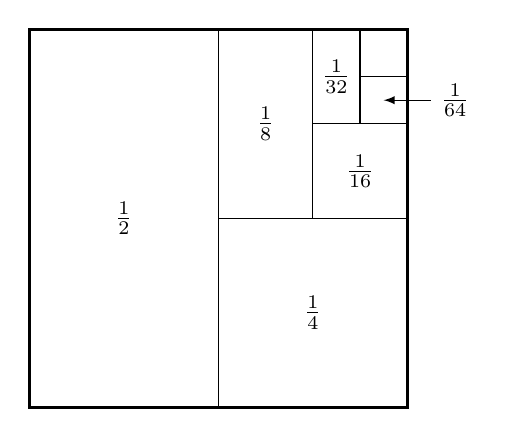
\begin{tikzpicture}[scale=.6,>=latex]
      \draw[very thick] (0,0) rectangle (8,8);
\draw(4,0)--(4,8);  \node at (2,4){$\frac{1}{2}$};
\draw (4,4)--(8,4); \node at (6,2){$\frac{1}{4}$};
\draw (6,4)--(6,8); \node at (5,6){$\frac{1}{8}$};
\draw (6,6)--(8,6); \node at (7,5){$\frac{1}{16}$};
\draw (7,6)--(7,8); \node at (6.5,7){$\frac{1}{32}$};
\draw (7,7)--(8,7); 
\draw[<-] (7.5,6.5)--(8.5,6.5)node[right] {$\frac{1}{64}$};
  \end{tikzpicture}
  \caption{}\label{fig:square}
\end{figure}
\[\frac{1}{2}+\frac{1}{4}+\frac{1}{8}+\frac{1}{16}+\frac{1}{32}+\cdots\]
从这个无穷级数里,依次取出前 $n$ 项的部分和 $S_n$, 得到数列 $\{s_n\}$:
\[s_1=\frac{1}{2},\quad s_2=\frac{1}{2}+\frac{1}{4}=\frac{3}{4},\quad s_3=\frac{1}{2}+\frac{1}{4}+\frac{1}{8}=\frac{7}{8},\ldots\]
\[s_n=\frac{1}{2}+\frac{1}{4}+\cdots+\frac{1}{2^n}=\frac{\dfrac{1}{2}\left[1-\left(\dfrac{1}{2}\right)^n\right]}{1-\dfrac{1}{2}}=1-\left(\frac{1}{2}\right)^n,\ldots\]

我们看到,这个数列 $\{s_n\}$ 和原正方形的关系是:
\begin{enumerate}
  \item 前 $n$ 项部分和 $s_n$ 小于1;
  \item $s_n$ 与 1 的误差 $|s_n-1|$, 只要 $n$ 充分大,就可以小到任意小。
\end{enumerate}
因此,前 $n$ 项部分和 $s_n$ 的极限是 1, 即
\[\lim_{n\to\infty} s_n=1 \]

我们可以这样理解无穷级数 $\sum\limits_{n=1}^{\infty}\dfrac{1}{2^n}$ 的意义,它就是前 $n$ 项部分和 $s_n$ 的极限值,于是
\[\frac{1}{2}+\frac{1}{4}+\frac{1}{8}+\cdots+\frac{1}{2^n}+\cdots=1 \]
我们说,这个无穷级数收敛到 1, 而前c$n$c项的部分和 $s_n$ 是这个极限的近似值。

现在,我们可以赋予这一类收敛的无穷级数以和的意义。

\begin{Definition}
  如果无穷级数 $u_1+u_2+\cdots+u_n+\cdots$ 的前 $n$ 项部分和 $s_n$ 所组成的数列 $\{s_n\}$ 有极限值,即 $\lim\limits_{n\to\infty}s_n=s$, 那么,这个无穷级数就叫做收敛的,并把这个确定的数 $\lim\limits_{n\to\infty}s_n=s$ 叫做这个无穷级数的和,即
\[\sum_{n=1}^{\infty}u_n=\lim_{n\to\infty}s_n=s\]
\end{Definition}
 
下面我们用收敛的数列来构造收敛的无穷级数。假设数列 $\{a_n\}$ 是收敛的,即$\lim\limits_{n\to\infty}a_n=A$, 令 $b_i=a_i-a_{i-1},\; i=1,2,\ldots$,即得一个新数列 $\{b_n\}$。无穷级数 $b_1+b_2+\cdots+b_n+b_{n+1}+\cdots$ 是收敛的。

事实上,这个级数的部分和是:
\[\begin{split}
    s_1&=b_1=a_1-a_0\\
    s_2&=b_1+b_2=(a_1-a_0)+(a_2-a_1)=a_2-a_0\\
    s_3&=b_1+b_2+b_3=(a_1-a_0)+(a_2-a_1)+(a_3-a_2)=a_3-a_0\\
    \cdots \\
    s_n&=b_1+b_2+\cdots +b_n=(a_1-a_0)+(a_2-a_1)+\cdots +(a_n-a_{n-1})=a_n-a_0\\
    \cdots \\
\end{split} \]
因此:
\begin{equation}
  \label{eq:infinity_series}
    \begin{split}
        \sum^{\infty}_{i=1}b_i&=\lim_{n\to\infty}\sum^n_{i=1}b_i=\lim_{n\to\infty}(a_n-a_0)\\
        &=\lim_{n\to\infty}a_n-a_0
    \end{split}
\end{equation}
因此,无穷级数 $\sum\limits^{\infty}_{i=1}b_i$ 是收敛的。


\begin{example}
令 $a_n=1-\dfrac{1}{n+1}$,$n=0,1,2,\ldots$,显然 $\{a_n\}$ 是收敛的,并且$\lim\limits_{n\to \infty}a_n=1$。

令\[\begin{split}
    b_i&=a_{i}-a_{i-1}=\left(1-\frac{1}{i+1}\right)-\left(1-\frac{1}{i}\right)\\
    &=\frac{1}{i}-\frac{1}{i+1}=\frac{1}{i(i+1)}
\end{split}\]
于是,      
\[\begin{split}
    \frac{1}{1\cdot 2}+\frac{1}{2\cdot 3}+\frac{1}{3\cdot 4}+\cdots +\frac{1}{n(n+1)}&=\lim_{n\to\infty}a_n-a_0\\
    &=\lim_{n\to\infty}\left(1-\frac{1}{n-1}\right)-0=1
\end{split}\]

上面\cref{eq:infinity_series} 也表示,要求一个无穷级数的和 $\sum\limits^{\infty}_{i=1}b_i$, 常将 $b_i$ 分解,使 $b_i=a_i-a_{i-1}$, 于是求无穷级数的和就转化为求数列 $\{a_n\}$ 的极限。
\end{example}

\begin{example}\label{exp:rational_series}
    求以下无穷等比级数的和。
    \[a_1+a_q+a_1q^2+\cdots +aq^{n-1}+\cdots \qquad (|q|<1)\]
\end{example}


\begin{solution}
    我们在本章中,已经证明,若 $|q|<1$,则 $\lim\limits_{n\to\infty}q^n=0$。因为:
\[s_n=\frac{a_1(1-q^n)}{1-q}=\frac{a_1}{1-q}-\frac{a_1q^n}{1-q}\]
所以,
\[\lim_{n\to\infty}s_n=\frac{a_1}{1-q}-\frac{a_1}{1-q}\lim_{n\to\infty}q^n=\frac{a_1}{1-q}\]
因此:\[a_1+a_q+a_1q^2+\cdots +aq^{n-1}+\cdots=\frac{a_1}{1-q} \quad (|q|<1)\]
\end{solution}

为了讨论循环小数及以后的需要,让我们用下面两个定理作为本节的总结。

\begin{Theorem}{定理1}
    无穷等比级数 $\sum\limits^{\infty}_{n=1}a_1q^{n-1}$ 收敛的充分必要条件是公比 $q$ 的绝对值 $|q|<1$,此时,它的和是 $\dfrac{a_1}{1-q}$,(注意这里 $q\neq 1$)。
\end{Theorem}

\begin{proof}
  上面的\cref{exp:rational_series} 已证明了 $|q|<1$ 是$\sum\limits^{\infty}_{n=1}a_1q^{n-1}=\dfrac{a_1}{1-q}$
的充分条件。要证必要性,我们只须注意到,如果 $|q|\geqslant 1$, 
那么 $a_n=a_1q^{n-1}$ 是发散的,于是,$\sum\limits^{\infty}_{n=1}a_1q^{n-1}$也是发散的(见下面的定理2)。
\end{proof}

\begin{Theorem}{定理2}
无穷级数 $\sum\limits^{\infty}_{i=1}a_i$ 收敛的必要条件是 $\lim\limits_{n\to \infty}a_n=0$.
\end{Theorem}

\begin{proof}
因为 $a_n=(a_1+a_2+\cdots +a_n)-(a_1+a_2+\cdots +a_{n-1})
=s_n-s_{n-1}$

由于 $\sum\limits^{\infty}_{i=1}a_i$ 是收敛的,故有
\[\begin{split}
    \lim_{n\to\infty}s_n&=\lim_{n\to\infty}s_{n-1}=s\\
    \lim_{n\to\infty}a_n&=\lim_{n\to\infty}(s_n-s_{n-1})=\lim_{n\to\infty}s_n-\lim_{n\to\infty}s_{n-1}=s-s=0
\end{split}\]
\end{proof}

下面的例题说明这个条件不是充分的。


\begin{example}
  $\displaystyle\frac{1}{1}+\frac{1}{2}+\frac{1}{3}+\cdots +\frac{1}{n}+\cdots$ 是发散级数,为什么呢?
\end{example}

\begin{solution}
  我们首先注意到这是正项级数,因此,部分和会越来越大,而且
\[\begin{split}
    s_1&=1          \\
    s_2&=1+\frac{1}{2}          \\
    s_4&=1+\frac{1}{2}+\frac{1}{3}+\frac{1}{4}>1+\frac{1}{2}+\frac{1}{4}+\frac{1}{4}=1+\frac{1}{2}+\frac{1}{2}          \\
    s_8&=1+\frac{1}{2}+\frac{1}{3}+\frac{1}{4}+\frac{1}{5}+\frac{1}{6}+\frac{1}{7}+\frac{1}{9}          \\
    &>1+\frac{1}{2}+\frac{1}{4}+\frac{1}{4}+\frac{1}{8}+\frac{1}{8}+\frac{1}{8}+\frac{1}{8}=1+\frac{1}{2}+\frac{1}{2}+\frac{1}{2}\\
    \cdots 
\end{split}\]

一般地,
\[s_{2^m}=1+\overbrace{\frac{1}{2}+\frac{1}{2}+\cdots +\frac{1}{2}}^{\text{$m$个}}=\frac{m+2}{2}\]    
{\linespread{1.5}\selectfont
因为,当 $m$ 无限增大时,$\dfrac{m+2}{2}$ 越来越大毫无止境,故 $s_{2^m}$ 也
发散到无穷大,又总有这样的 $n$ 满足 $2^m<n$, 故当 $m\to\infty$ 时,
也使 $m\to\infty$, $s_n>s_{2^m}\to \infty$, 即 $s_n$ 也发散到无穷大。\par}

注意到:$a_n\to 0$, 但如果数列 $\{s_n\}$中的子数列$\{s_{2^m}\}$ 是
发散的,那么 $\{s_n\}$ 也是发散的。
\end{solution}

\subsection{无限小数与十分逼近}
在这一节,我们要用无限十进小数来描述实数,要说明无限小数的意义,证明每一个循环小数都等于一个分数,而每一个分数都等于一个循环小数。

现在我们借助十分逼近法去规定实数的无限十进小数表示。考察某实数 $x$。将数轴分为单位线段,各分点均为整数。点 $x$ 在某一线段内,或者本身就是一个分点。如果 $x$ 是相邻两个单位线段的分点,约定 $x$ 属于线段的左端点。于是,存在一个整数 $\alpha_0$,使得
\[\alpha_0\le x<\alpha_0+1,\quad \text{即}\; x\in \overline{A_0B_0}=(\alpha_0,\alpha_0+1)\]

{\linespread{1.6}\selectfont$\displaystyle \alpha_0+\frac{1}{10},\; \alpha_0+\frac{2}{10},\; \alpha_0+\frac{3}{10},\;\ldots,\; \alpha_0+\frac{9}{10}$ 这些点将 $\overline{A_0B_0}=(\alpha_0,\alpha_0+1)$ 分为十等份,点 $x$ 必在某一个分段内,或者 $x$ 本身是一个分点,如果是分点,约定 $x$ 属于分段的左端
点,在这两种情况下,存在一个整数 $\alpha_1,\; (0\leqslant \alpha_1\leqslant 9)$,使得\par}
\[\alpha_0+\frac{\alpha_1}{10}\le x<\alpha_0+\frac{\alpha_1+1}{10}\]
即:$\displaystyle x\in\overline{A_1B_1}=\left[\alpha_0+\frac{\alpha_1}{10}, \alpha_0+\frac{\alpha_1+1}{10}\right)$。

\medskip
再将线段 $\overline{A_1B_1}$十等分,我们可以找到一个整数 $\alpha_2$($0\leqslant \alpha_2\leqslant 9$),使得
\[\alpha_0+\frac{\alpha_1}{10}+\frac{\alpha_2}{10^2}\le x<\alpha_0+\frac{\alpha_1+1}{10}+\frac{\alpha_2+1}{10^2}\]
即:$\displaystyle x\in\overline{A_2B_2}=\left[\alpha_0+\frac{\alpha_1}{10}+\frac{\alpha_2}{10^2}, \alpha_0+\frac{\alpha_1+1}{10}+\frac{\alpha_2+1}{10^2}\right)$。

经过 $n$ 步以后,$x$ 必在线段 $\overline{A_nB_n}$ 之中,即
\[\alpha_0+\frac{\alpha_1}{10}+\frac{\alpha_2}{10^2}+\cdots+\frac{\alpha_n}{10^n}\le x<\alpha_0+\frac{\alpha_1}{10}+\frac{\alpha_2}{10^2}+\cdots+\frac{\alpha_n+1}{10^n}\]
这里 $\alpha_1,\alpha_2,\ldots,\alpha_n$ 都是 0 到 9 之间的整数,线段$\overline{A_nB_n}$ 之长度等于 $\dfrac{1}{10^n}$,而有限十进小数$\alpha_0.\alpha_1\alpha_2\cdots\alpha_n$ 和 $\alpha_0.\alpha_1\alpha_2\cdots(\alpha_n+1)$ 分别是 $x$ 的准确到 $\dfrac{1}{10^n}$ 的不足近似值和过剩近似值。

让这个十分逼近过程无限地进行下去,那么实数 $x$ 就完全可以由无限小数$\alpha_0.\alpha_1\alpha_2\cdots\alpha_n\cdots$ 来表示,同时由于 $x$ 与有限
小数近似值的误差
\[|\alpha_0.\alpha_1\alpha_2\cdots\alpha_n-x|<\frac{1}{10^n},\qquad  |\alpha_0.\alpha_1\alpha_2\cdots(\alpha_n+1)-x|<\frac{1}{10^n}\]
当 $n$ 充分大时,可以小到任意小,所以无限小数 $x=\alpha_0.\alpha_1\alpha_2\cdots\alpha_n\cdots$ 是由有限十进小数组成的两个数列:
\[\alpha_0,\; \alpha_0.\alpha_1,\;\alpha_0.\alpha_1\alpha_2,\;\ldots,\;  \alpha_0.\alpha_1\alpha_2\cdots\alpha_n,\;\ldots\]
与
\[(\alpha_0+1),\; \alpha_0.(\alpha_1+1),\;\alpha_0.\alpha_1(\alpha_2+1),\;\ldots, \alpha_0.\alpha_1\alpha_2\cdots(\alpha_n+1),\;\ldots\]
的共同的极限值。

\emph{无限小数的定义}是这样的,我们取实数的小数点以下第 $n$ 位为止的有限小数 $\alpha_0.\alpha_1\alpha_2\cdots\alpha_n$,记作 $x_n$,即 $x_n=\alpha_0.\alpha_1\alpha_2\cdots\alpha_n$,那么数列 $\{x_n\}$ 的极限值是这个无限小数,用式子表示就是
\[\lim_{n\to\infty}x_n=x=\alpha_0.\alpha_1\alpha_2\cdots\alpha_n\cdots\]


\begin{example}
$\dfrac{2}{3}=0.\dot{6}$表示数列$\{x_n\}$的极限:
\[x_1=0.6,\; x_2=0.66,\; x_3=0.666,\ldots,\; x_n=0.\underbrace{66\cdots 66}_{\text{$n$位小数}},\; \ldots\]
\end{example}

\begin{example}
  无限小数 $\uppi=3.1415926\cdots$ 的意思是,令
  \[ x_1=3.1,\; x_2=3.14,\; x_3=3.141,\; \ldots\]
  那么 $x_n\to \uppi$。
\end{example}

注意,在上面我们用十分逼近得到实数 $x$ 的无限十进小数表示时,在 $x$ 是十等分的一个分点的情形,如果不限定 $x$ 属于两相邻线段的左端点,那么对于同一个整数或有限小数,可能有两类不同的无限十进小数表示法。例如
\[1=1.0000\cdots=0.999\cdots,\quad 2.35=2.35000\cdots=2.34999\cdots\]

为排除这种不确定性,按照我们的约定,就可以去掉那些从某一位以后有数字都是 9 的十进小数表达式。

把实数写成小数形式,便于比较它们的大小。在比较时,遇到以 9 为循环节结尾的无限小数都用以 0 为循环节结尾的无限小数代替。

今有两个实数 $x=\alpha_0.\alpha_1\alpha_2\cdots\alpha_n\cdots$ 和 $y=\beta_0.\beta_1\beta_2\cdots\beta_n\cdots$,比较这两个实数 $x$ 和 $y$ 的大小,只须比较两个数的各数位上的数字,并且注意在哪一个数位上的数字不同,从而告诉我
们哪个实数大。


{\linespread{1.6}\selectfont 例如:$\dfrac{17}{20}=0.850000\cdots$,$\dfrac{45}{53}=0.84905000\cdots$,看一眼就能发觉,它们有相同的第一位小数,$\frac{17}{20}$ 的第二位小数大于 $\frac{45}{53}$ 的第二位小数,因此,$\dfrac{17}{20}>\dfrac{45}{53}$。\par}

\medskip
一般地,我们说 $x>y$,如果下面的条件中有一个成立
\begin{enumerate}
  \item $\alpha>\beta$
  \item $\alpha=\beta$,而 $\alpha_1>\beta_1$
  \item $\alpha=\beta, \alpha_1 =\beta_1,\ldots,\alpha_{\ell}=\beta_{\ell}$,而 $\alpha_{\ell+1}>\beta_{\ell+1}$
\end{enumerate}

\bigskip
根据前面的讨论,我们知道任何一个实数都是两个有限十进小数的夹逼数列的极限。

设 $\lim x_n=x=\lim x'_n,\quad \lim y_n=y=\lim y'_n$,或者
\[x_n\to x\leftarrow x'_n,\qquad y_n\to y\leftarrow y'_n\]
\[x'_n-x_n\to 0,\qquad y'_n-y_n\to 0\]
则对应数列的相加,我们有实数的相加,对应于数列相乘,我们有实数的相乘,也就是说:
\[\begin{split}
  \lim(x_n+y_n)&=x+y=\lim(x'_n+y'_n)\\
  \lim(x_n\cdot y_n)&=x\cdot y=\lim(x'_n\cdot y'_n)
\end{split}
\]

例如 $\sqrt{2}=1.4142135\cdots,\quad \sqrt{3}=1.7320508\cdots$,
\[\begin{cases}
    x_n+y_n\\  x'_n+y'_n
\end{cases}\qquad \begin{cases}
    1.4+1.7=3.1 \\ 1.5+1.8=3.3
\end{cases}\]
\[\begin{cases}
    1.41+1.73=3.14\\1.42+1.74=3.16
\end{cases}\qquad \begin{cases}
    1.414+1.732=3.146\\1.415+1.733=3.148
\end{cases}\]
\[\begin{cases}
    1.4142+1.7320=3.1462\\
1.4143+1.7321=3.1464
\end{cases}\qquad \begin{cases}
    1.41421+1.73205=3.14626\\
1.41422+1.73206=3.14628
\end{cases}\cdots\]
即:
$3.1 <3.14<3.146<3.1462<3.14626<\cdots <\sqrt{2}+\sqrt{3}<\cdots <3.14628<3.1464<3.148<3.16<3.3$

$\therefore\quad \sqrt{2}+\sqrt{3}=3.1462\cdots$。只要把 $\sqrt{2}$, $\sqrt{3}$ 的夹逼小数求到足够多的数位,我们用上面的方法就可以把 $\sqrt{2}+\sqrt{3}$ 的小数表示求到任意的数位上。

同样地得到
\[\begin{cases}
    x_n\cdot y_n\\  x'_n\cdot y'_n
\end{cases}\qquad \begin{cases}
    1.4\times 1.7=2.38 \\ 1.5\times 1.8=2.70
\end{cases}\qquad \begin{cases}
    1.41\times 1.73=2.4393\\1.42\times 1.74=2.4708
\end{cases}\]
\[\begin{cases}
    1.414\times 1.732=2.449048\\1.415\times 1.733=2.452195
\end{cases}\qquad \begin{cases}
    1.4142\times 1.7320=2.4493944\\
1.4143\times 1.7321=2.449709
\end{cases}\cdots\]

$\therefore\quad \sqrt{6}=2.449\cdots$。

在无限小数中,除了有一类\emph{无限循环小数},还有一类\emph{无限不循环小数},譬如,$0.1001000100001\cdots$,就是一个无限不循环小数。

现在我们要来证明每一个循环小数都等于一个分数,而每一个分数都等于一个循环小数。先举几个将无限循环小数化为分数的例子,再给出一般的证明。

\begin{example}
  怎样将循环小数 $0.\overline{621}$ 化成分数?
\end{example}

\begin{solution}
  我们可以将无限小数 $0.\overline{621}$ 表示成一个无穷级数
\[\begin{split}
0.\overline{621}&=0.621+0.000621+0.000000621+\cdots\\
&=\frac{621}{10^3}+\frac{621}{10^6}+\frac{621}{10^9}+\cdots
\end{split}\]
显然,这个无穷级数是无穷等比级数,它的首项 $a_1=\dfrac{621}{10^3}$, 公比$q=\dfrac{1}{10^3}$ 根据 4.1 中的定理,这个无穷等比级数的和是 $\dfrac{a_1}{1-q}$,因此:
\[\begin{split}
    0.\overline{621}&=\frac{621}{10^3}+\frac{621}{10^6}+\frac{621}{10^9}+\cdots\\
    &=\frac{621}{10^3}\cdot \frac{1}{1-\frac{1}{10^3}}=\frac{621}{10^3}\cdot \frac{10^3}{10^3-1}\\
    &=\frac{621}{999}=\frac{23}{37}
\end{split}\]
\end{solution}

\begin{example}
试将$0.3\overline{12}$化成分数。
\end{example}

\begin{solution}
\[\begin{split}
    0.3\overline{12}&= 0.3+0.0\overline{12}=0.3+(0.012+0.00012+\cdots)\\
    &=\frac{3}{10}+\left(\frac{12}{10^3}+\frac{12}{10^5}+\cdots\right)\\
    &=\frac{3}{10}+\frac{12}{10^3}\cdot \frac{1}{1-\dfrac{1}{10^2}}\\
    &=\frac{3}{10}+\frac{12}{10^3}\cdot \frac{10^2}{10^2-1}\\
    &=\frac{3}{10}+\frac{12}{10}\cdot \frac{1}{99}=\frac{309}{990}=\frac{103}{330}
\end{split}\]
\end{solution}

下面,我们来证明任何一个循环小数一定是一个分数。

如果 $a$ 是个循环小数,它的循环节是由第 $k+1$ 位开始到 $k+\ell$ 位,平常我们写作
\[a=a_0.c_1c_2\cdots c_k\overline{c_{k+1}c_{k+2}\cdots c_{k+\ell}}\]
它的意思是
\[\begin{split}
    a&=a_0+\frac{c_1}{10}+\frac{c_2}{10^2}+\cdots +\frac{c_k}{10^k}+\frac{c_{k+1}}{10^{k+1}}+\cdots+\frac{c_{k+\ell}}{10^{k+\ell}}\\
&\qquad +\frac{c_{k+1}}{10^{k+\ell+1}}+\cdots+\frac{c_{k+\ell}}{10^{k+2\ell}}+\frac{c_{k+1}}{10^{k+2\ell+1}}+\cdots+\frac{c_{k+\ell}}{10^{k+3\ell}}+\cdots
\end{split}\]

虽然,这不是无穷等比级数,现在用结合律来构造这个无穷级数的部分和的子数列:

设 $S_1=a_0+\dfrac{c_1}{10},\quad S_2=a_0+\dfrac{c_1}{10}+\dfrac{c_2}{10^2},\ldots$ 于是第 $k$ 个部分和是
\[S_k=a_0+\frac{c_1}{10}+\frac{c_2}{10^2}+\cdots+\frac{c_k}{10^k}\]
再令
\[d=\frac{c_{k+1}}{10^{k+1}}+\frac{c_{k+2}}{10^{k+2}}+\cdots +\frac{c_{k+\ell}}{10^{k+\ell}}\]
所以,$d$ 是分数,而且 $0\leqslant d<1$。

那么,第 $k+m\ell$ 个部分和是
\[\begin{split}
    S_{k+m\ell}&=S_k+d+\frac{d}{10^{\ell}}+\frac{d}{10^{2\ell}}+\cdots \frac{d}{10^{(m-1)\ell}}\\
    &=S_k+d\left(1+\frac{1}{10^{\ell}}+\frac{1}{10^{2\ell}}+\cdots +\frac{1}{10^{(m-1)\ell}}\right)\\
    &=S_k+\frac{d\left(1-\dfrac{1}{10^{m\ell}}\right)}{1-\dfrac{1}{10^{\ell}}}
\end{split}\]
当 $m=1,2,3,\ldots$ 时,部分和 $S_{k+m\ell}$ 就构成无穷级数的部分和数列 $\{S_n\}$ 的子数列 $\{S_{k+m\ell}\}$, 并且
\[\begin{split}
    \lim_{m\to\infty}S_{k+m\ell}&= \lim_{m\to\infty}\left\{S_k+\frac{d\left(1-\frac{1}{10^{m\ell}}\right)}{1-\frac{1}{10^{\ell}}}\right\}\\
    &=S_k+\frac{d}{1-\frac{1}{10^{\ell}}}=S_k+\frac{10^{\ell}\cdot d}{10^{\ell}-1}=a'
\end{split}\]
这里 $a'$ 表示分数。我们只证明了部分和数列的子数列 $\{S_{k+m\ell}\}$ 收敛到分数
$a'$,还需要证明部分和数列 $\{S_n\}$ 也收敛到 $a'$。

我们只须注意到原来的循环小数所代表的无穷级数也都是正项的,这就是说,部分和数列$\{S_n\}$是递增数列,特别地,如果 $k+m\ell\leqslant n<k+(m+1)\ell$,
那么 $S_{k+m\ell}\leqslant S_n\leqslant S_{k+(m+1)\ell}$,因此,如果“子数列” $\{S_{k+m\ell},\; m=1,2,3,\ldots\}$ 收敛到 $a'$, 原数列 $\{S_n\}$也收敛到 $a'$。

我们已证明了,每个循环小数都可以化为分数,现在证明分数可以化为循环小数。

设 $\dfrac{a}{b}$ 为一任意给定的不可约真分数(亦即 $a,b$ 互质且 $a<b$)。

\medskip
\begin{enumerate}
  \item $b$ 只含有 2 或 5 的质因子,则容易看出可以化 $\dfrac{a}{b}$ 成有限位小数。

事实上,设 $b=2^{\alpha}5^{\beta}$, $d=5^{\alpha-\beta}a$,若 $\alpha\geqslant \beta$,则
\[\frac{a}{b}=\frac{a}{2^{\alpha}5^{\beta}}=\frac{5^{\alpha-\beta}a}{10^{\alpha}}=\frac{d}{10^{\alpha}}\]
为 $\alpha$ 位小数。我们可以把有限位小数看成循环小数的特例。如:
\[\frac{1237}{2\times 5^3}=\frac{1237\times 2^2}{10^3}=4.948=4.948\overline{0}\]

\item\label{itm:proof_fraction_step2} 设 $b$ 与 10 互质,即:$(b,10)=1$, 根据整数分解的唯一性而知 $\dfrac{a}{b}$ 不可能写成 $\dfrac{m}{10^k}$ 的形式,这里 $m$ 为正整数,故 $\dfrac{a}{b}$ 不可能化为有限小数。做除法,我们得到
\[10a=bq_1+r_1,\qquad 0<r_1<b\]
两边再除以 $b$,得
\[\frac{10a}{b}=q_1+\frac{r_1}{b},\qquad 0<\frac{r_1}{b}<1\]

这里 $q$ 是 $0,1,2,\ldots,9$ 这十个整数中的某个。用和上面同样的方法,逐步得到
\[\begin{split}
    \frac{10r_1}{b}&=q_2+\frac{r_2}{b},\qquad 0<\frac{r_2}{b}<1,\\
    \frac{10r_2}{b}&=q_3+\frac{r_3}{b},\qquad 0<\frac{r_3}{b}<1,\\
\cdots  \\
    \frac{10r_{n-1}}{b}&=q_n+\frac{r_n}{b},\qquad 0<\frac{r_n}{b}<1\\
\end{split}\]
这里每个 $q_n$ 是 $0,1,2,\ldots,9$ 这十个整数中的某个,于是
\[\begin{split}
    \frac{a}{b}&=\frac{q_1}{10}+\frac{r_1}{10b}\\
    &=\frac{q_1}{10}+\frac{q_2}{10^2}+\frac{r_2}{10^2b}\\
    &=\frac{q_1}{10}+\frac{q_2}{10^2}+\frac{q_3}{10^3}+\frac{r_3}{10^3b}\\
    \cdots  \\
    &=\frac{q_1}{10}+\frac{q_2}{10^2}+\cdots+\frac{q_n}{10^n}+\frac{r_n}{10^n b}\\
\end{split}\]

再设
\[\begin{split}
    x_n&=\frac{q_1}{10}+\frac{q_2}{10^2}+\cdots+\frac{q_n}{10^n}\\
    y_n&=\frac{q_1}{10}+\frac{q_2}{10^2}+\cdots+\frac{q_n+1}{10^n}\\
    d_n&=\frac{r_n}{10^n b}<\frac{1}{10^n}
\end{split}\]
则:
\[\frac{a}{b}=x_n+d_n,\qquad 0<d_n<\frac{1}{10^n}\]

再有 $x_1<x_2<\cdots<x_{n-1}<x_n<\cdots<y_n<y_{n-1}<\cdots<y_2<y_1$,且 $y_n-x_n\to 0$。

当 $n$ 无限增大时,根据实数完备性,无限小数
\[\sum_{n=1}^{\infty}\frac{q_n}{10^n}=0.q_1q_2\cdots q_n\cdots\]
为一实数,又因为 $d_n\to 0$,故我们确定了一个其值为 $\dfrac{a}{b}$ 的无限小数 $0.q_1q_2\cdots q_n\cdots$。

\medskip
{\linespread{1.4}\selectfont
再说明这个无限小数一定是纯循环小数,设 $a=r_0$, 因为
$r_0,r_1,r_2,\ldots,r_n,\ldots$ 是一串大于 0 而小于 $b$ 的正整数,这种正整数只有 $b-1$ 个不同的,所以,这一串数 $r_0=a,r_1,r_2,\ldots r_n,\ldots$ 必然有二者会相同,就假定 $r_k$ 为首先出现的重见余数,假定这两个相同的余数是 $r_k$ 和 $r_i$, 即有 $r_k=r_i$。现在我们要证明 $r_i$ 只能是 $a=r_0$,用反证法,若 $i>0$ 则由等式
$\dfrac{10r_{k-1}}{b}=q_k+r_k$ 和 $\dfrac{10r_{i-1}}{b}=q_i+r_i$ 两边作减法,得到\par}
\[\frac{10(r_{k-1}-r_{i-1})}{b}=q_k-q_i\]
因为 $q_k-q_i$ 是整数,所以 $b$ 能整除 $10(r_{k-1}-r_{i-1})$,由于 $b$ 与 10
互质,故 $b$ 能整除 $r_{k-1}-r_{i-1}$,但是 $r_{k-1}-r_{i-1}<b$,所以 $r_{k-1}-r_{i-1}=0$,即 $r_{k-1}=r_{i-1}$ 重见更早,与原设 $r_k$ 为首先出现的重见余数不合,故 $i=0$。

$\therefore\quad r_k=r_0=a$, 这样
\[\frac{a}{b}=0.\overline{q_1q_2\cdots q_{k-1}q_k}\]

\item 设 $b=2^{\alpha}5^{\beta}b_1$, 而 $b_1>1$ 且与 10 互质,又 $\alpha$ 与 $\beta$ 均不为 0, 若 $\alpha\geqslant \beta$,
\[\frac{a}{b}=\frac{a}{2^{\alpha}5^{\beta}b_1}=\frac{5^{\alpha-\beta}a}{10^{\alpha}b_1}\]
做 $5^{\alpha-\beta}a$ 除以 $b_1$,得
\[5^{\alpha-\beta}a=M{b_1}+{r},\quad 0<r<b\]
$M$ 是一个正整数,两边再除以 $b_1$,得
\[5^{\alpha-\beta}\frac{a}{b_1}=M+\frac{r}{b_1},\qquad 0<\frac{r}{b_1}<1\]
由前段证明 \ref{itm:proof_fraction_step2} 的结果
\[\frac{r}{b_1}=0.\overline{c_1c_2\cdots c_{s}}\]
故,
\[\begin{split}
    \frac{a}{b}&=\frac{5^{\alpha-\beta}a}{10^{\alpha}b_1}=\frac{1}{10^{\alpha}}\left(M+0.\overline{c_1c_2\cdots c_{s}}\right)\\
    &=\frac{1}{10^{\alpha}}\left(M.\overline{c_1c_2\cdots c_{s}}\right)
\end{split}\]

当以 $10^{\alpha}$ 除以 $M.\overline{c_1c_2\cdots c_{s}}$ 时,也就是将小数点左移$\alpha$ 位,我们得到
\[\frac{a}{b}=0.m_1m_2\cdots m_{\alpha}\overline{c_1c_2\cdots c_{s}}\]
为混循环小数。
\end{enumerate}

若 $\alpha\le \beta$,可以用同样的方法说明 $\dfrac{a}{b}$ 为一混循环小数,因
此有
\begin{Theorem}{定理}
    任何一个分数都等于某一个循环小数,任何一个循环小数必然是个分数。
\end{Theorem}

如果采用无限十进小数来描述实数,我们按照下表来对实数分类:
\[\text{实数——无限十进小数}\begin{cases}
    \text{有理数—无限十进循环小数}\\
    \text{无理数—无限十进不循环小数}
\end{cases}\]

\begin{Exercise}
\begin{question}
    \item 求下列无穷等比数列的和:
  \begin{tasks}(2)
    \task $\displaystyle \frac{1}{2}+\frac{1}{3}+\frac{2}{9}+\cdots$
    \task $\displaystyle 1-\frac{2}{5}+\frac{4}{25}-\cdots$
    \task $\displaystyle \sqrt{\frac{3}{2}}+\sqrt{\frac{2}{3}}+\frac{2}{3}\sqrt{\frac{2}{3}}+\cdots$
    \task $\displaystyle \frac{\sqrt{3}+1}{\sqrt{3}-1}+1+\frac{\sqrt{3}-1}{\sqrt{3}+1}+\cdots$
  \end{tasks}        
  \item 若 $a,b$ 是实数且 $\left|\dfrac{a+2b+3}{b+3}\right|+3(a+3b)^2=0$, 求等比级数 $ab+b+\dfrac{b}{a}+\cdots$ 的和。
  \item 已知 $\sqrt{3}\sin\alpha-\cos\alpha=0$, $\alpha$ 为锐角,求 $\sum\limits^{\infty}_{n=0}(-\sin\alpha)^n$
  \item 求下列无穷级数的和:
  \begin{tasks}
    \task $\displaystyle \frac{1}{1 \times 4}+\frac{1}{2 \times 5}+\frac{1}{3 \times 6}+\frac{1}{4 \times 7}+\cdots$
    \task $\displaystyle \frac{6}{2 \times 7}+\frac{6}{7 \times 12}+\frac{6}{12 \times 17}+\frac{6}{17 \times 22}+\cdots$
    \task $\displaystyle \frac{1}{1 \times 2 \times 3}+\frac{1}{2 \times 3 \times 4}+\frac{1}{3 \times 4 \times 5}+\frac{1}{4 \times 5 \times 6}+\cdots$
    \task $\displaystyle \frac{1}{1 \times 2 \times 3 \times 4}+\frac{1}{2 \times 3 \times 4 \times 5}+\frac{1}{3 \times 4 \times 5 \times 6}+\frac{1}{4 \times 5 \times 6 \times 7}+\cdots$
    \task $\displaystyle \frac{1}{7}+\frac{2}{7^{2}}+\frac{3}{7^{3}}+\frac{1}{7^{4}}+\frac{2}{7^{6}}+\frac{3}{7^{6}}+\frac{1}{7^{7}}+\frac{2}{7^{8}}+\frac{3}{7^{9}}+\cdots$
  \end{tasks}
  \item 求下列各式的极限值:
  \begin{tasks}
      \task $\displaystyle \lim _{n\to  \infty} \frac{1+a+a^{2}+\cdots+a^{n}}{1+b+b^{2}+\cdots+b^{n}} \qquad(|a|<1,\;|b|<1)$
      \task $\displaystyle \lim _{n\to  \infty}\left(\frac{1}{n}-\frac{2}{n}+\frac{3}{n}-\cdots+\frac{(-1)^{n-1} n}{n}\right)$
      \task $\displaystyle \lim _{n\to  \infty}\left(\frac{1^{2}}{n^{3}}+\frac{2^{2}}{n^{3}}+\cdots+\frac{(n-1)^{2}}{n^{3}}\right)$
      \task $\displaystyle \lim _{n\to  \infty}\left(\frac{1}{2}+\frac{3}{{2^2}}+\frac{5}{2^3}+\cdots+\frac{2n-1}{2^{n}}\right)$
  \end{tasks}
  \item $\displaystyle \lim_{n\to  \infty}\left(1-\frac{1}{2^2}\right)\left(1-\frac{1}{3^2}\right)\left(1-\frac{1}{4^2}\right)\cdots\left(1-\frac{1}{n^2}\right)$
  \item 数列 $x_n\; (n=1,2,3,\ldots)$ 是由下列各式所确定:
\[x_0=a,\; x_1=b,\; x_n=\frac{x_{n-2}+x_{n-1}}{2}\quad (n\ge 2)\]
求 $\lim\limits_{n\to\infty}x_n$.
  \item 将下列循环小数化为分数:
  \[0.\overline{47},\qquad 2.\overline{234},\qquad 0.4\overline{7},\qquad 3.2\overline{31},\qquad 0.\overline{1108},\qquad 5.38\overline{90}\]
  \item 求出下列各式的值:
  \begin{tasks}(2)
    \task $0.\overline{48}\times0.\overline{48}$
    \task $0.\overline{12}+0.\overline{83}+0.\overline{34}+\cdots+0.\overline{89}$
    \task $0.\overline{15}+0.0\overline{15}+0.00\overline{15}+\cdots$
  \end{tasks}
\end{question}
\end{Exercise}

\section{数列极限在几何上的应用}
在平面几何中,我们知道了什么是相似形,而且知道研究相似形的基本定理是“设 $\triangle ABC$ 和 $\triangle A'B'C'$ 的三个内角对应相等,则其对应边长成比例”。在初中时,我们证明了当比值是有理数时,定理是对的,现在要补充推证,在比值是无理数时,定理也是对的,这样这个定理的证明才是完整的。

\begin{proof}
设 $AB=kA'B'$, 这里 $k$ 是无理数,我们要证明
\[\frac{AC}{A'C'}=\frac{BC}{B'C'}=k\]
我们知道任何一个无理数可以用有理数来逼近,于是可以找到两串有理数 $k'_n,k''_n$ 从左、右夹逼无理数 $k$ 使得
\[k'_n\to k\leftarrow k''_n,\quad \text{或者}\quad \lim_{n\to\infty}k'_n=\lim_{n\to\infty}k''_n=k\]
比如,$k$ 是特殊的情形,$k=\sqrt{2}$,则可取
\[\begin{split}
    k'_1&=1,\quad     k'_2=1.4,\quad    k'_3=1.41,\;\ldots\\ 
    k''_1&=1,\quad     k''_2=1.5,\quad    k''_3=1.42,\;\ldots\\
\end{split}\]

\begin{figure}
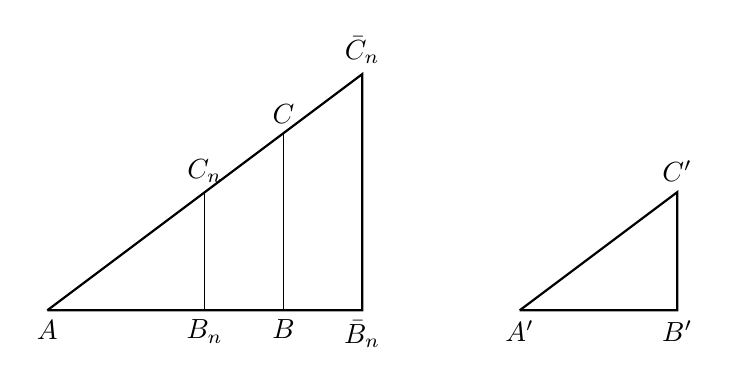
\begin{tikzpicture}
\begin{scope}
  \draw[thick] (0,0)node[below]{$A$}--(4,0)node[below]{$\bar{B}_n$}--(4,3)node[above]{$\bar{C}_n$}--(0,0);
  \draw(3,0)node[below]{${B}$}--(3,2.25)node[above]{$C$};
  \draw(2,0)node[below]{${B}_n$}--(2,1.5)node[above]{${C}_n$};
\end{scope}
\begin{scope}[xshift=6cm]
\draw[thick] (0,0)node[below]{$A'$}--(2,0)node[below]{$B'$}--(2,1.5)node[above]{$C'$}--(0,0);
\end{scope}
\end{tikzpicture}
    \caption{}\label{fig:sim_ratio}
\end{figure}

如\cref{fig:sim_ratio},在直线 $AB$ 上取点列 $\{B_n\}$和$\{\bar{B}_n\}$ 使得
\[AB_n=k'_nA'B',\qquad A\bar{B}_n=k''_n A'B'\]
再由 $B_n$, $\bar{B}_n$点 分别作 $BC$ 边平行线交 $AC$ 线于 $C_n$,$\bar{C}_n$点,则因为相似三角形定理对有理数比值是对的,所以
\[\triangle AB_nC_n \sim \triangle A\bar{B}_n\bar{C}_n \sim \triangle A'B'C'\]
\[\begin{split}
  \frac{AB_n}{A'B'}&=\frac{AC_n}{A'C'}=\frac{B_nC_n}{B'C'}=k'_n\\
  \frac{A\bar{B}_n}{A'B'}&=\frac{A\bar{C}_n}{A'C'}=\frac{\bar{B}_n\bar{C}_n}{B'C'}=k''_n\\
\end{split}\]
由作图知
\[k'_nA'B'=AB_n<AB<A\bar{B}_n=k''_nA'B'\]
并可得
\[\begin{split}
     k'_nA'C'&=AC_n<AC<A\bar{C}_n=k''_nA'C'\\
k'_nB'C'&=B_nC_n<BC<\bar{B}_n\bar{C}_n=k''_nB'C'
\end{split}\]
对上面不等式各端取极限,得到
\[\lim_{n\to\infty} k'_n A'C'  =  \lim_{n\to\infty}k''_n A'C'   =kA'C'\]
另一方面又可得到
\[\lim_{n\to\infty} k'_n A'C' = \lim_{n\to\infty}k''_n A'C'  =AC\]
根据数列的极限值是唯一的,因此 $AC=kA'C'$,同理可得
$BC=kB'C'$。
\end{proof}

\bigskip
总结上面的证明可以归纳成下面两点:
\begin{enumerate}
  \item 先有一个数 $k$, 因为它是无理数,比较复杂,往往我们要用简单的有理数逐步逼近它;
  \item 在求极限过程中,要点是要用极限值的唯一性保证所要的结论。
\end{enumerate}

\medskip
在几何上,$\uppi$ 表示单位圆的面积,这个面积 显然能用一个有理数或无理数来表示,可是,如果我们想要以任何精确度计算出数元,这个定义对于我们来说并没有什么帮助。这
时,我们必须借助于求极限的过程,把数 $\uppi$ 表示为已知并且不难算出的数列的极限,除此外别无它法。

假如我们把单位圆等分成 $2n$ 个小扇形,然后一上一下间插排列起来,如\cref{fig:divide_circle}。
\begin{figure}
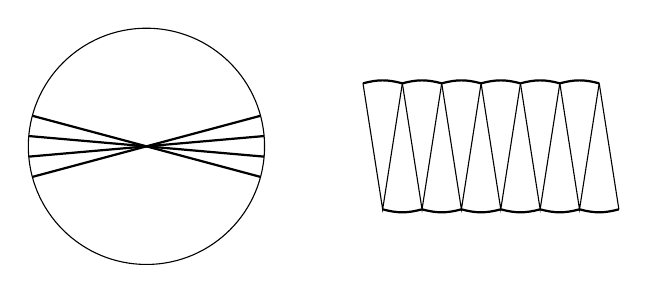
\begin{tikzpicture}
\begin{scope}
    \draw (0,0) circle (1.5);
    \foreach \x in {15,-5,5,-15}
    {
        \draw[thick] (\x:1.5)--(\x+180:1.5);
    }
\end{scope}
\begin{scope}[xshift=3cm]
    \foreach \x in {0,.5,1,...,2.5}
    {
        \draw[thick] (\x,-.8) to[bend right=15] (\x+.5,-.8);
        \draw[thick] (\x-.25,.8) to[bend right=-15] (\x+.25,.8);
        \draw[smooth] (\x+.25,.8)--(\x,-.8)--(\x-.25,.8) ;
    }
    \draw[smooth] (3,-.8)--(3-.25,.8) ;
\end{scope}
\end{tikzpicture}
    \caption{}\label{fig:divide_circle}
\end{figure}

当 $n$ 愈大时,上图就愈接近一个高为 1, 面积为 $\uppi$ 的矩形。这也就说明了单位圆的圆周长等于 $2\uppi$。

早在三国时代,我国古代数学家刘徽于公元 263 年在《九章算术》中,对古率 $\uppi=3$ 极为不满,就提出了用折线逐步地来逼近曲线,用正多边形的面积来逐步地逼近圆的面积的思想,他说如果圆内接正六边形,正十二边形,二十四边形……依次递求它的面积,边数愈增多则其面积与圆面积 愈加接近,如果边数增加到无限则多边形面积的极限就与圆面积相等。

设 $\uppi$ 为单位圆面积,$S_n$ 为单位圆的内接正 $n$ 边形的面积,$S$ 为单位圆的外切正 $n$ 边形的面积,如\cref{fig:polygon_circle},对于每一个 $n$,从几何直观上作如下估计
\begin{figure}
\begin{tikzpicture}[>=latex, scale=1.8]
\draw (0,0) circle (1);
\draw[thick] (30:1)--(90:1)--(150:1)--(210:1)--(270:1)--(330:1)--(30:1);
\draw [thick](0:1.165)--(60:1.165)--(120:1.165)--(180:1.165)--(240:1.165)--(300:1.165)--(0:1.165);
\draw (0,0)node[left]{$O$}--(0:1.165);
\draw  (-30:1)--(0,0)-- (30:1);
\draw[|<->|] (1.8,0) --node[right]{$\sin\dfrac{\uppi}{n}$}(1.8,.5);
\draw (.25,0) arc (0:30:.25)node[right]{$\uppi/n$}; 
\draw[|<->|] (1.26,0) --node[right]{$\tan\dfrac{\uppi}{n}$}(30:1.1);
\node at (42:.5){1};
\end{tikzpicture}   
    \caption{}\label{fig:polygon_circle}
\end{figure}

$S_n<S_{2n}<\uppi<S'_{2n}<S'_n$, 
刘徽的计算理论基础是,$|S_n-\uppi|<S'_n-S_n$, 在 $n$ 无限增大时,$(S'_n-S_n)\to 0$。从\cref{fig:polygon_circle} 看出:
\[\begin{split}
    S'_n&=2n\text{直角三角形的面积}=2n\cdot \frac{1}{2}\tan\frac{\uppi}{n}=n\tan\frac{\uppi}{n}   \\
    S_n&=2n\text{直角三角形的面积}=2n\cdot \frac{1}{2}\cos\frac{\uppi}{n}\cdot \sin \frac{\uppi}{n}=n\sin\frac{\uppi}{n}\cdot \cos\frac{\uppi}{n}
\end{split}\]

\[\begin{split}
    S'_n-S_n &= n\left(\tan\frac{\uppi}{n}-\sin\frac{\uppi}{n}\cdot \cos\frac{\uppi}{n}\right)\\
    &=n \sin\frac{\uppi}{n}\left(\frac{1}{\cos\dfrac{\uppi}{n}}-\cos\frac{\uppi}{n}\right)\\
    &=\frac{1}{2}(\text{圆内接 $n$ 边形周长})\left(\frac{1}{\cos\dfrac{\uppi}{n}}-\cos\frac{\uppi}{n}\right)\\
    &<\frac{1}{2}(\text{圆外切六边形周长})\left(\frac{1}{\cos\dfrac{\uppi}{n}}-\cos\frac{\uppi}{n}\right)\to 0\\
\end{split} \]

这就说明了由圆内接正多边形的面积所组成的数列 $\{S_{6\cdot 2^{n-1}}\}$ 的极限是 $\uppi$. 

让我们计算这个数列中的前面几个面积。面积的通项是
\[S_{6\cdot 2^{n-1}}=6\cdot 2^{n-1}\left(\frac{1}{2}\sin\frac{\uppi}{3\cdot 2^{n-1}}\right)=3\cdot 2^{n-1}\sin\frac{\uppi}{3\cdot 2^{n-1}}\quad (n=1,2,3,\ldots)\]

为由 $\sin\dfrac{\uppi}{n}$ 求出 $\sin\dfrac{\uppi}{2n}$,我们需要导出它们之间的递推关系:
\[\begin{split}
    \sin\frac{\uppi}{2n}&=\sqrt{\frac{1-\cos\dfrac{\uppi}{n}}{2}}\\
    &=\frac{1}{2}\sqrt{2-2\cos\frac{\uppi}{n}}\\
    &=\frac{1}{2}\sqrt{2-2\sqrt{1-\sin^2\frac{\uppi}{n}}}
\end{split}\]
于是:
\begin{itemize}[itemsep=5pt]
    \item 当 $n=1$, $S_6=3\cdot \sin \dfrac{\uppi}{3}=2.5980762$, 
    \item 当 $n=2$, $S_{12}=6\cdot \sin \dfrac{\uppi}{6}=3$,
    \item 当 $n=3$, 
    \[\begin{split}
        S_{24}&=12\cdot \sin \frac{\uppi}{12}=12\left(\frac{1}{2}\sqrt{2-2\sqrt{1-\left(\frac{1}{2}\right)^2}}\right)\\
        &=12\cdot \left(\frac{1}{2}\sqrt{2-\sqrt{3}}\right)=12\times 0.258819=3.1058285
    \end{split}\]
    \item 当 $n=4$, 
    \[\begin{split}
        S_{48}&=24\cdot \sin \frac{\uppi}{24}=24\left(\frac{1}{2}\sqrt{2-2\sqrt{1-0.258819^2}}\right)\\
        &=24\times 0.1305266=3.132639
    \end{split}\]
    \item 当 $n=5$, 
    \[\begin{split}
        S_{96}&=48\cdot \sin \frac{\uppi}{48}=48\left(\frac{1}{2}\sqrt{2-2\sqrt{1-0.1305266^2}}\right)\\
        &=48\times 0.0654031=3.1393515
    \end{split}\]
    \item 当 $n=6$, 
    \[\begin{split}
        S_{192}&=96\cdot \sin \frac{\uppi}{96}=96\left(\frac{1}{2}\sqrt{2-2\sqrt{1-0.0654031^2}}\right)\\
        &=96\times 0.032719=3.1410307
    \end{split}\]
\end{itemize}

现在我们对 $\uppi$ 的近似值 $S_{192}\approx 3.1410307$ 的误差作如下估计
\[\begin{split}
    |S_{192}-\uppi|&<192\left(\tan\frac{\uppi}{192}-\frac{1}{2}\sin\frac{\uppi}{96}\right)\\
    &=192\left(0.0163639-\frac{1}{2}\times 0.032719\right)\\
    &=0.000845
\end{split}\]
刘徽定 $\uppi\approx 3.14$,后世称之为\emph{徽率},在\emph{刘徽}以后重新推算圆周率贡献最大的是南朝\emph{祖冲之}(公元429—500年)。祖冲之的著名结果为
\[3.1415926<\uppi <3.1415927\]
\[\text{密率}\,\uppi=\frac{355}{113},\qquad \text{约率}\,\uppi=\frac{22}{7}\]
全世界定圆周率值准确到 $\dfrac{1}{10^7}$ 的,当推\emph{祖冲之}为第一人。


\begin{Exercise}
\begin{question}
  \item 联结三角形 $ABC$ 三边的中点 $D,E,F$, 作三角形 $DEF$, 再联结 $\triangle DEF$ 各边之中点,作 $\triangle GHI$,如此下去,求所得一切三角形面积之总和与原三角形面积之比。
  \item 从 $\angle BAC$ 边上一点 $B$ 起,作 $BC\bot AC$,从 $C$ 作 $CD\bot AB$,从 $D$ 再作 $DE \perp AC$, 这样无限继续下去,设 $BC=\qty{7}{cm}$,$CD=\qty{6}{cm}$,求这些垂线的和(\cref{fig:question_triangle})。
  \item 有一束射线,每相邻两条射线间的夹角为 $\alpha$,从一条射线上任一点对其紧邻的一射线作垂线 $S_0$,从它的垂足再对下一射线作垂线 $S_1$,依此类推(\cref{fig:question_ratio})。问:$\lim\limits_{n\to\infty} (S_0+S_1+S_2+\cdots +S_n+\cdots )$
  \begin{figurehere}
    \begin{minipage}[t]{0.48\textwidth}
      \centering
      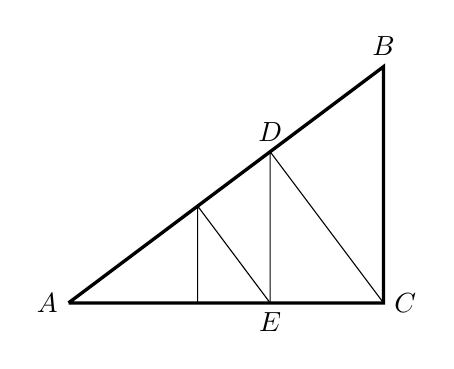
\begin{tikzpicture}[>=latex, scale=1]
        \draw[very thick] (0,0)node[left]{$A$}--(4,0)node[right]{$C$}--(4,3)node[above]{$B$}--(0,0);
        \draw (4,0)--(2.56,1.92)node[above]{$D$}--(2.56,0)node[below]{$E$};
        \draw (2.56,0)--(1.64,1.23)--(1.64,0);
      \end{tikzpicture}
      \caption{}\label{fig:question_triangle}
    \end{minipage}
    \begin{minipage}[t]{0.48\textwidth}
      \centering
      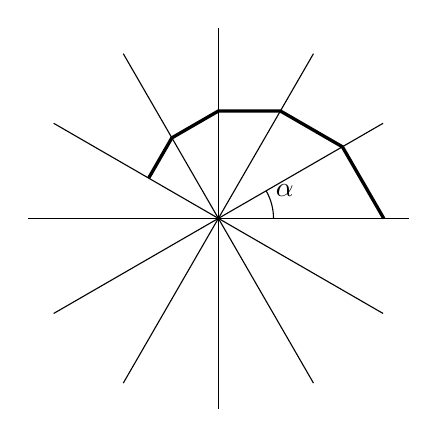
\begin{tikzpicture}[>=latex, scale=.7]
        \foreach \x in {0,1,2,...,11}
        {
            \draw(0,0)--(30*\x:3.45);
        }
        \draw[very thick] (3,0)--(30:0.866*3)--(60:0.866*0.866*3)--(90:0.866*0.866*0.866*3)--(120:0.866*0.866*0.866*0.866*3)--(150:0.866*0.866*0.866*0.866*0.866*3);
        \draw (1,0) arc (0:30:1)node [right]{$\alpha$};
      \end{tikzpicture}
      \caption{}\label{fig:question_ratio}
    \end{minipage}
  \end{figurehere}
  \item 直角三角形三边之长分别为 $3,4,5$,作一圆内切于此三角形,再作一圆外切于此圆,并切于三角形的斜边和边长为 4 的直角边,如此继续作下去,则得到一个切圆的序列,求这些圆的面积之和。
\end{question}
\end{Exercise}

\section{数列极限存在定理}
前面在引进数列极限的定义时,所考虑的许多数列的极限都是已经知道的,然后再用数列极限的定义来验证,如果数列极限的概念仅能给出这样的认识,即一些已知数能够用另一些已知数的某些数列来逼近,那么我们从极限概念所得到的东西太少了。但是数列的一个最为重要的应用在于,有些问题所要确定的数值往往不能用别的方法直接得知或表示,却能用数列极限方式来表示。例如我们用有理数逼近无理数,又在上一节用圆内接正多边形的面积来逼近圆面积,求出 $\uppi$ 的数值等,这样的例子就是数列极限重要应用的典型例子。因此我们构造的数列是否收敛就成为第一位重要问题了。对于一个数列 $\{a_n\}$ 的极限,事实上应该分成两个层次来讨论。

\begin{enumerate}
  \item 存在性。即数列 $\{a_n\}$ 是否有极限存在?
  \item 求值问题。假如已经确定了给定数列 $\{a_n\}$ 的极限存在,我们再设法求它的极限值,其实只要确定了 $\{a_n\}$ 的极限存在,那么这个极限值就是一个实数,而数列 $\{a_n\}$ 就是它的逐次逼近的近似数值,要点是去了解数列的性质,总之求值问题是个比较次要的问题了。 
\end{enumerate}

下面给出一个比较简单的极限存在定理。
\begin{Theorem}[极限存在定理]{定理}
  递增有上界的数列 $\{a_n\}$ 极限存在(同样,递减有下界数列 $\{a_n\}$ 的极限也存在)。
\end{Theorem}
 
{\linespread{1.65}\selectfont
例如:数列 $\left\{\dfrac{n^2-1}{n^2}\right\}$ 符合定理的条件,因为 
$0,\; \dfrac{3}{4},\; \dfrac{8}{9},\; \dfrac{15}{16},\; \dfrac{24}{25},\; \ldots$ 显然是递增的,同时 $a_n=\dfrac{n^2-1}{n^2}=1-\dfrac{1}{n^2}<1$, 也就是说,它是有界的,而且容易看出数列的极限值是 1,事实上\par}
\[\lim_{n\to\infty}\frac{n^2-1}{n^2}=\lim_{n\to\infty}\left(1-\frac{1}{n^2}\right)=1-0=1\]

下面的证明可以说是将二分逼近和实数完备性配合运用的典型例子,在这儿是初次用到,往后还会遇到相似的配合用法。其实,只要能基本上理解命题意义和证明大意,就可以先去学习它的应用,往往用了几次后再回头看第二遍,也就更加明白了。

\begin{proof}
  一个使得 $a_n\leqslant K$ 恒成立的常数 $K$ 叫做 $\{a_n\}$ 的一个\emph{上界}。下面我们将用二分逼近法和完备性来说明 $\{a_n\}$ 的极限等于它的\emph{最小上界}(因为 $\{a_n\}$ 是递增的)。

{\linespread{1.65}\selectfont 令 $A_1=a_1$,$B_1=K$,由假设 $A_1=a_1\leqslant a_n\leqslant K=B_1$,即所有 $a_n$ 都在线段 $[A_1,B_1]$ 之内,将线段 $[A_1,B_1]$ 二等分,假如分点 $\dfrac{1}{2}(A_1+B_1)$ 还是一个上界(即 $a_n\leqslant \dfrac{A_1+B_1}{2}$ 恒成立),则取前半段为 $[A_2,B_2]$,不然则取后半段为 $[A_2,B_2]$。这样逐次二等分,每次当分点 $\dfrac{1}{2}(A_m+B_m)$ 是一个上界时,取其前半段,不然则取其后半段,继续不断地按照上述办法二等分而选取其半段,就得到满足下列性质的两个夹逼数列 $\{A_n\}$ 和 $\{B_n\}$:\par}

\begin{enumerate}
  \item\label{itm:property1} $A_1\leqslant A_2\le A_3\leqslant \cdots \leqslant A_m\leqslant \cdots \leqslant B_m\le \cdots\leqslant B_3\leqslant B_2\leqslant B_1$,$(B_m-A_m)\to 0$
  \item\label{itm:property2} 所有 $B_m$ 都是数列 $\{a_n\}$ 的上界。
  \item\label{itm:property3} 对于任何 $A_m$, 都至少有一个 $a_N$ 使得 $A_m<a_N$,换言之,线段 $[A_m,B_m]$ 至少包含一个点,比如 $a_N$(由 $\{a_n\}$ 的递增性,所有 $n\geqslant N$ 也满足 $A_m<a_n$)。
\end{enumerate}

因此,由性质 \ref{itm:property1} 和实数完备性就得到唯一的实数 $k$,介于一切 $A_m$ 和 $B_m$ 之间,换言之,存在唯一实数 $k$ 使得  $\lim_{m\to\infty}A_m=k=\lim_{m\to\infty}B_m$

现在让我们来说明 $k$ 也就是 $\{a_n\}$ 的极限!设 $\varepsilon$ 是一个任给的正数,因为 $\lim\limits_{m\to\infty}A_m=k=\lim\limits_{m\to\infty}B_m$,所以存在足够大的 $M$, 使得(如\cref{fig:k_between_A_B})
\begin{equation}
    k-\varepsilon<A_M\le k\le B_M<k+\varepsilon
\end{equation}
\begin{figure}
  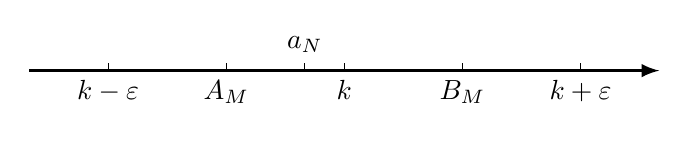
\begin{tikzpicture}[>=latex]
        \draw[very thick,->] (1,0)--(9,0);    
\foreach \x/\xtext in {5/k,2/k-\varepsilon,8/k+\varepsilon,3.5/A_M,6.5/B_M}
{
    \draw (\x,0)node[below]{$\xtext$}--(\x,.1);
}    
\draw (4.5,0)--(4.5,.1)node[above]{$a_N$};
    \end{tikzpicture}

    \caption{}\label{fig:k_between_A_B}
\end{figure}
由性质 \ref{itm:property3} 知道,存在一个够大的 $N$,使得
\begin{equation}
    A_M<a_N    
\end{equation}
由性质 \ref{itm:property2} 知道,$B_M$ 是一个上界,即恒有
\begin{equation}
    a_N\leqslant B_M
\end{equation} 
由 $\{a_n\}$ 的递增性,当 $n\geqslant N$ 时,有
\begin{equation}
    a_N\leqslant a_n
\end{equation}

综合上述四点,就说明了当 $n\geqslant N$时,有
\[k-\varepsilon<A_M\le a_N\le a_n<B_M<k+\varepsilon\]
亦即 $|a_n-k|<\varepsilon$, 这也就说明了 $\lim\limits_{n\to\infty}a_n=k$。
\end{proof}


\begin{example}
  应用本节存在定理,求 $\displaystyle \lim_{n\to\infty}\frac{r^n}{n!}$。
\end{example}

\begin{solution}
    设 $x_n=\dfrac{r^n}{n!}$,则
\[x_{n+1}=\frac{|r|}{n+1}|x_n|\]
所以只在 $n>|r|-1$ 时,数列 $\{|x_n|\}$ 才是递减的,同时,由于 $|x_n|>0$,所以它是有下界的,因此数列 $\{|x_n|\}$ 收敛于 $\ell$,在上面等式两边取极限
\[\lim_{n\to\infty}|x_{n+1}|=\lim_{n\to\infty}\frac{|r|}{n+1}\cdot |x_n|\]
即
\[\lim_{n\to\infty}|x_{x+1}|=\lim_{n\to\infty}\frac{|r|}{n+1}\cdot \lim_{n\to\infty}|x_n|\]
因为变量 $|x_{n+1}|$ 和 $|x_n|$ 取同一个数列的数值(除第一个数值外)。因此有同一个极限 $\ell$,即:$\ell=0\cdot \ell$,所以
\[\lim_{n\to\infty}|x_n|=\ell=0\]
最后有
\[\lim_{n\to\infty} x_n=\lim_{n\to\infty} \frac{r^n}{n!} =0\]
\end{solution}

\begin{example}
    求下面数列$\{a_n\}$:
\[\begin{split}
   &  a_1=\sqrt{2},\quad a_2=\sqrt{2+\sqrt{2}},\quad a_3=\sqrt{2+\sqrt{2+\sqrt{2}}},\\
    & \ldots,\quad a_n=\underbrace{\sqrt{2+\sqrt{2+\cdots+\sqrt{2}}}}_{\text{$n$个根号}},\quad\ldots
\end{split} \]
的极限。
\end{example}
   
\begin{solution}
显然,$a_1=\sqrt{2},\;a_2=\sqrt{2+a_1},\;\ldots,\;
a_n=\sqrt{2+a_{n-1}},\;\ldots$

$\because\quad 2+\sqrt{2}>2,\qquad \therefore\quad a_2=\sqrt{2+\sqrt{2}}>\sqrt{2}=a_1$

又假设 $a_n>a_{n-1}$ 成立,则 $2+a_n>2+a_{n-1}$

$\therefore\quad a_{n+1}=\sqrt{2+a_n}>\sqrt{2+a_{n-1}}=a_n$

因此,对于一切 $n\in\mathbb{N}$,有 $a_{n+1}>a_n$,则此数列是递增的。

$\because\quad \sqrt{2}<2,\qquad \therefore\quad a_1<2,\quad a_2<\sqrt{2+2}=2$

假设 $a_{n-1}<2$,那么,
\[a_n=\sqrt{2+a_{n-1}}<\sqrt{2+2}=2\]
所以对于一切 $n\in\mathbb{N}$, 有 $a_n<2$ 。

根据极限存在定理知数列 $\{a_n\}$ 有极限,设它为 $x$,于是,
$\lim\limits_{n\to\infty}a_n=x$。
由于
\[a_n=\sqrt{2+a_{n-1}}\]
两边平方得
\[a^2_n={2+a_{n-1}}\]
取极限有
\[\lim_{n\to\infty}a^2_n =\lim_{n\to\infty}(2+a_{n-1})\]
或者:$x^2=2+x$,解得:
\[x_1=2,\qquad x_2=-1\]
然而 $\because\quad a_n>0\quad \Longrightarrow\quad \lim\limits_{n\to\infty}a_n=x\geqslant 0$,$\therefore\quad x_2=-1$ 不合要求,因此,
\[\lim_{n\to\infty}a_n=2\]
\end{solution}

由上面的极限存在定理可以引出下面的结论:
\begin{enumerate}
  \item 预先证明极限存在是很重要的,它也给实际计算这个极限提供了基础。
  \item 在极限定义中,要求我们预先猜到 $\{a_n\}$ 的极限值 $A$, 然后再用数列极限定义来验证这个极限 $A$ 是存在的,这就和前面所说的在数列极限的重要应用中出现的层次有些本末倒置,本节的极限存在定理就纠正了这种本末倒置的局面。
\end{enumerate}

\begin{Exercise}
\begin{question}
  \item 试利用关于单调而有界的数列的极限存在定理检验下面数列极限存在性。
  \begin{tasks}
    \task $a_n=1+\dfrac{1}{1\cdot 2}+\dfrac{1}{1\cdot 2\cdot 3}+\cdots+\dfrac{1}{1\cdot 2\cdot 3\cdots (n-1)}$,\quad $n=1,2,3,\ldots$
    \task $a_n=\dfrac{1}{n+1}+\dfrac{1}{n+2}+\cdots +\dfrac{1}{2n}$,\quad $n=1,2,3,\ldots$
    \task $x_n=p_0+\dfrac{p_1}{10}+\cdots +\dfrac{p_n}{10^n}$,式中 $p_i,\; (i=0,1,2,\ldots)$ 是非负数,且从 $p_1$ 起不大于 9。
  \end{tasks}
  \item 已知 $a_1=\sqrt{2},\; a_2=\sqrt{2\sqrt{2}},\; a_3=\sqrt{2\sqrt{2\sqrt{2}}},\ldots,a_{n+1}=\sqrt{2a_n},\ldots$, 求 $\lim\limits_{n\to\infty}a_n$。
  \item 设 $a_{n+1}=\sqrt{k+a_n}$, 这里 $k>0$,$a_1>0$,求证数列 $\{a_n\}$ 递增,并以方程 $x^2=x+k$ 的正根为极限。
  \item 已知 $x_1=1,x_2=1+\dfrac{x_1}{1+x_1},\ldots,x_n=1+\dfrac{x_{n-1}}{1+x_{n-1}},\ldots$, 求 $\lim\limits_{n\to\infty}x_n$。
  \item 数列 $\{x_n\}$ 由下面递归方程定义
  \[x_1=h,\qquad x_{n+1}=x_n^2+k\]
  这里 $0<k<\dfrac{1}{4}$,$h$ 在方程 $x^2-x+k=0$ 的二根 $a,b$ 之间,即 $a<h<b$。求证:$a<x_{n+1}<x_n<b$,并求 $\lim\limits_{n\to\infty}x_n$。
  \item 设 $0<a_1<b_1$ 是两个给定正数,令 
  \[\begin{split}
    a_2&=\sqrt{a_1b_1},\qquad b_2=\frac{1}{2}(a_1+b_1),\quad (a_2<b_2)\\
    a_3&=\sqrt{a_2b_2},\qquad b_3=\frac{1}{2}(a_2+ b_2),\quad (a_3<b_3)\\
    \cdots \\
    a_{n+1}&=\sqrt{a_nb_n},\qquad b_{n+1}=\frac{1}{2}(a_n+b_n),\quad (a_{n+1}<b_{n+1})\\
  \end{split}\]
  求证:
  \begin{tasks}
    \task $\{a_n\}$ 递增和 $\{b_n\}$ 递减;
    \task $\{a_n\}$ 和 $\{b_n\}$ 的极限相同。
  \end{tasks}
\end{question}
\end{Exercise}